\documentclass[../index.tex]{subfiles}

\begin{document}
    \section{Công cụ và thư viện sử dụng}
    \begin{table}[h]
        \centering
        \begin{tabular}{ |p{4cm}|p{5cm}|p{4.5cm}| }
            \hline
            Công cụ            & Mục đích          & URL                                \\
            \hline
            Jetbrains Rider    & C\# .NET IDE      & jetbrains.com/rider    \\
            \hline
            Jetbrains DataGrip & IDE Databases     & jetbrains.com/datagrip \\
            \hline
            Jetbrains Webstorm & Javascript IDE    & jetbrains.com/webstorm \\
            \hline
            Neovim             & Text Editor       & neovim.io                  \\
            \hline
            Postman            & API Platform      & postman.com            \\
            \hline
            Docker Desktop     & Docker Management & docker.com             \\
            \hline
            Cloudinary         & Cloud Storage     & cloudinary.com             \\
            \hline
            PrimeNG         & Thư viện UI Components     & primeng.org             \\
            \hline
            TailwindCSS         & CSS Framework     & tailwindcss.com             \\
            \hline
            Chart.js         & Thư viện UI vẽ biểu đồ     & chartjs.org             \\
            \hline
            Quill.js         & Thư viện UI text editor     & quilljs.com             \\
            \hline
        \end{tabular}
        \caption{Công cụ sử dụng}
    \end{table}
    Với sự trợ giúp của các công cụ và thư viện trên, em đã có thể xây dựng các ứng dụng và sản phẩm nhanh chóng và hiệu quả hơn. Các công cụ như Jetbrains IDE cung cấp môi trường phát triển và triển khai ổn định, giúp tiết kiệm thời gian và nâng cao năng suất. Các thư viện như PrimeNG, TailwindCSS và 1 số thư viện UI khác cung cấp các tính năng và chức năng sẵn có, giúp tập trung vào việc xây dựng các tính năng chính của ứng dụng thay vì phải tự code từ đầu. Sự kết hợp của các công cụ và thư viện này giúp em xây dựng được các ứng dụng chất lượng cao, với thời gian và chi phí hiệu quả hơn.

    \section{Minh họa ứng dụng trên giao diện}

    \subsection{UI Đăng nhập}
    \begin{figure}[H]
        \centering
        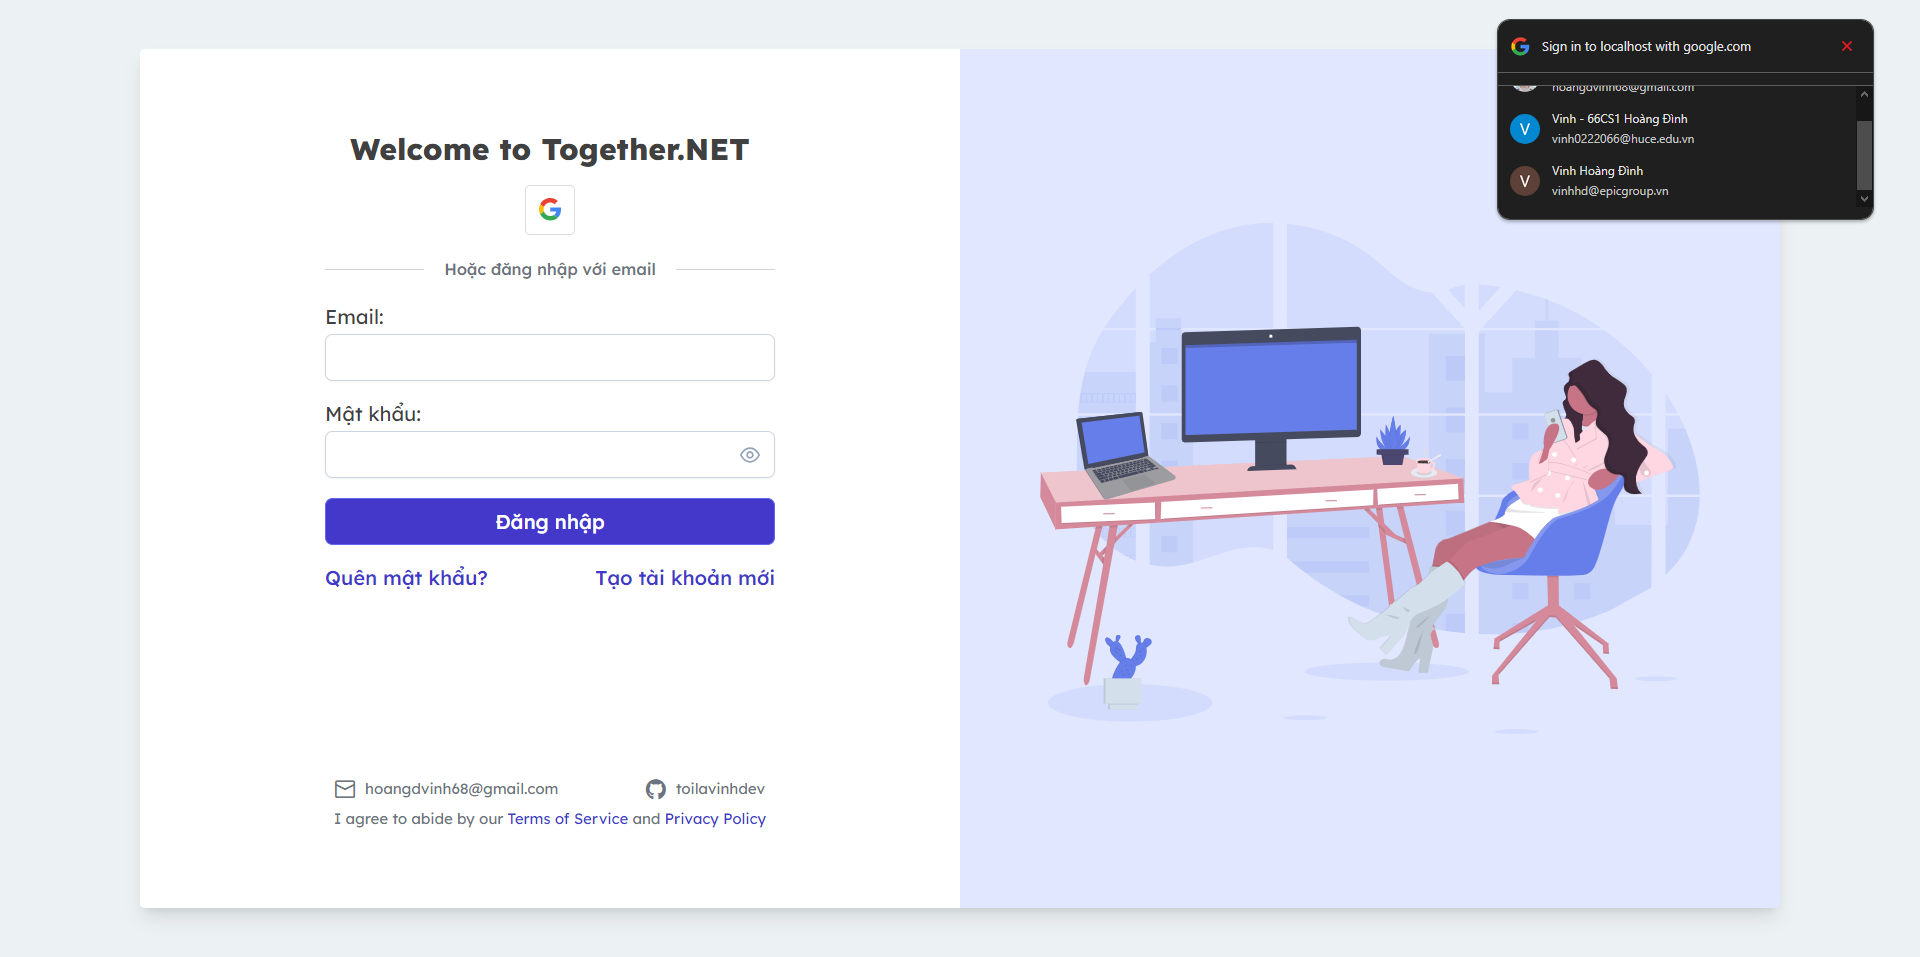
\includegraphics[width=1\linewidth]{figures/demo/sign-in-page}
        \caption{UI Đăng nhập}
    \end{figure}
    Màn hình đăng nhập của Together.NET có thiết kế đơn giản và hiện đại. Bên trái
    là form thông tin đăng nhập cùng nút "Đăng nhập" nổi bật. Dưới form có liên
    kết "Quên mật khẩu?" giúp người dùng dễ dàng khôi phục thông tin đăng nhập.

    \subsection{UI Đăng ký}
    \begin{figure}[H]
        \centering
        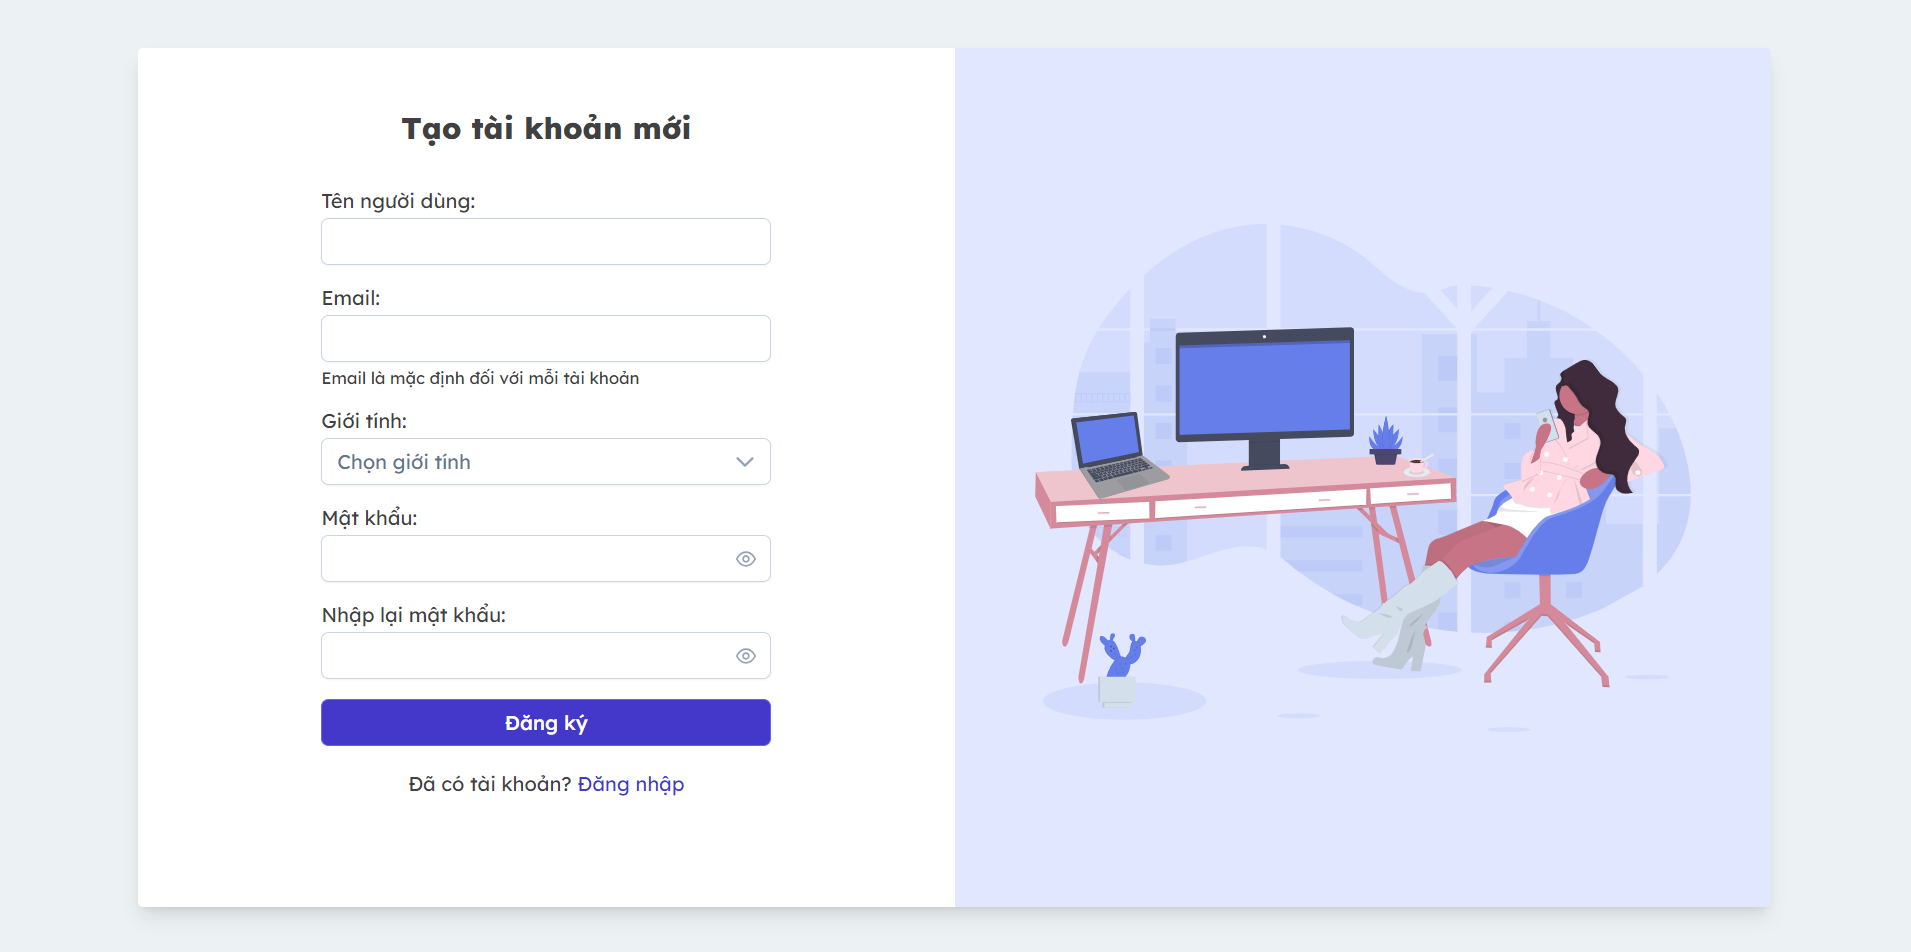
\includegraphics[width=1\linewidth]{figures/demo/sign-up-page}
        \caption{UI Đăng ký}
    \end{figure}
    Màn hình đăng ký tương tự như màn hình đăng nhập, thay vào đó là form đăng
    ký tạo tài khoản mới.

    \subsection{UI Trang chính diễn đàn}
    \begin{figure}[H]
        \centering
        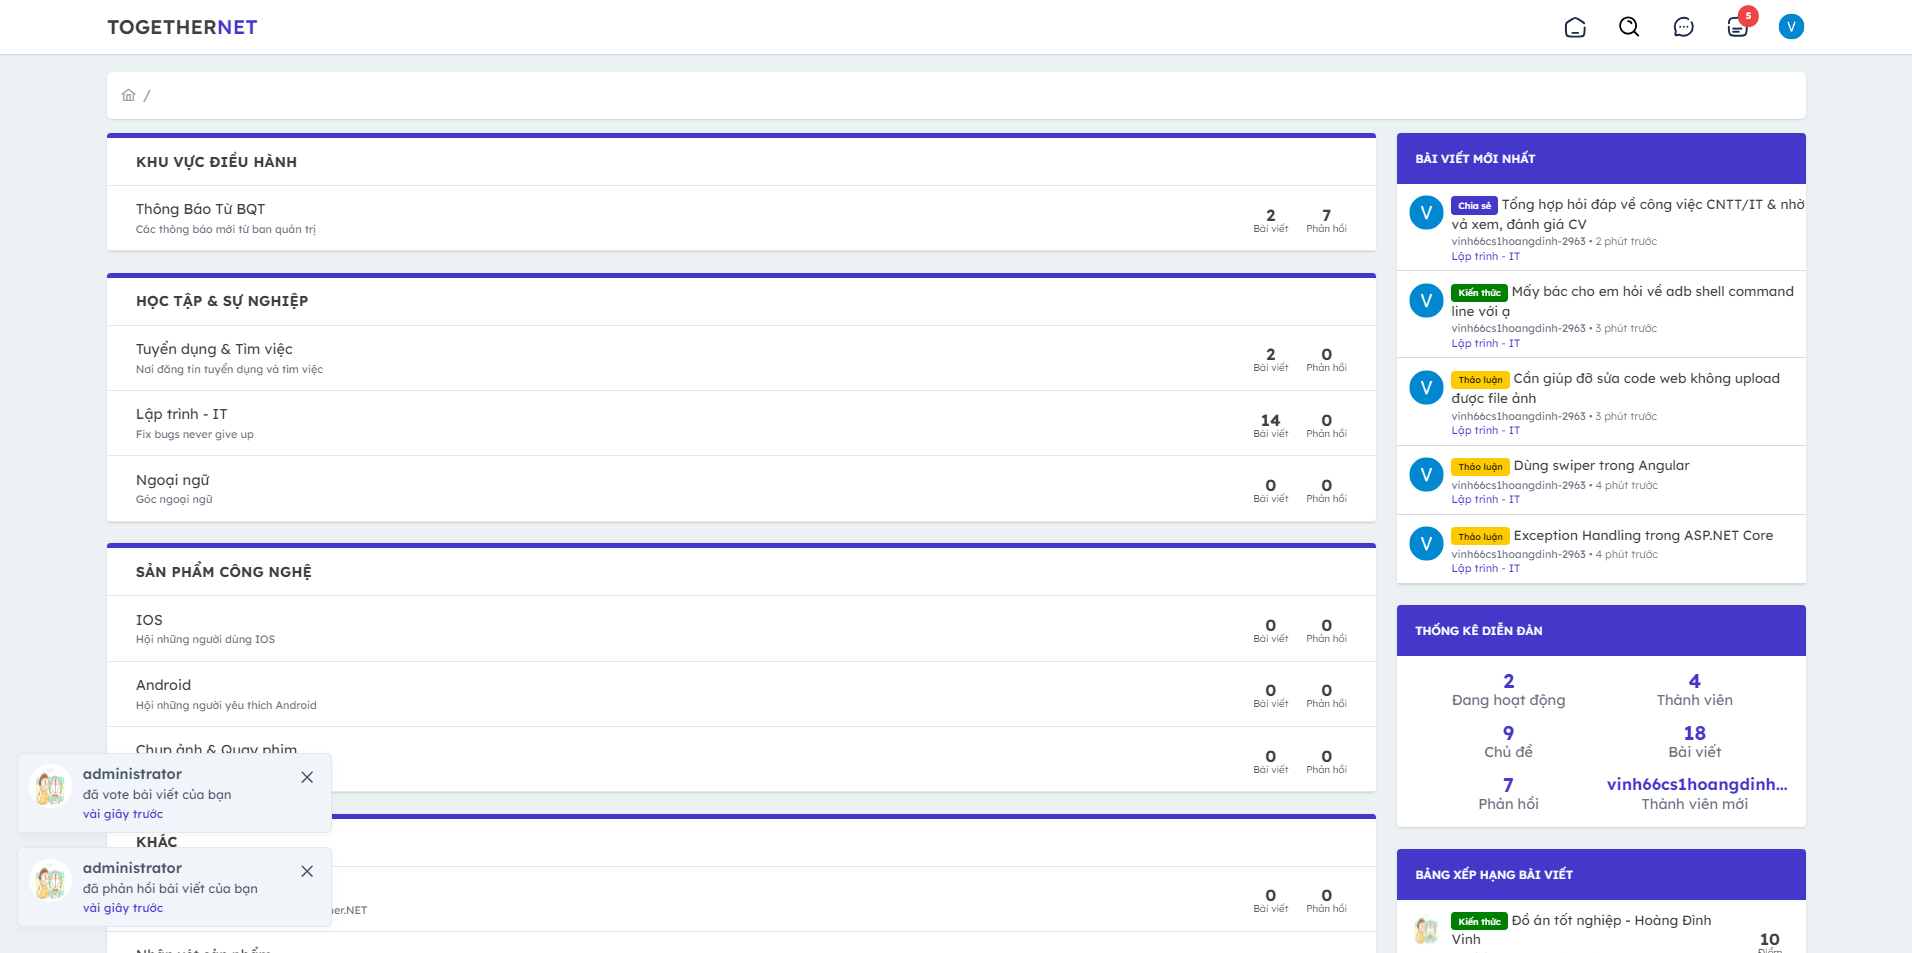
\includegraphics[width=1\linewidth]{figures/demo/home-page}
        \caption{UI Trang chính diễn đàn}
    \end{figure}
    Màn hình trang chính hiển thị các diễn đàn với bố cục rõ ràng. Người dùng có
    thể dễ dàng duyệt qua các chủ đề, tham gia thảo luận và truy cập nhanh các
    tính năng trên thanh header.

    \subsection{UI Chủ đề}
    \begin{figure}[H]
        \centering
        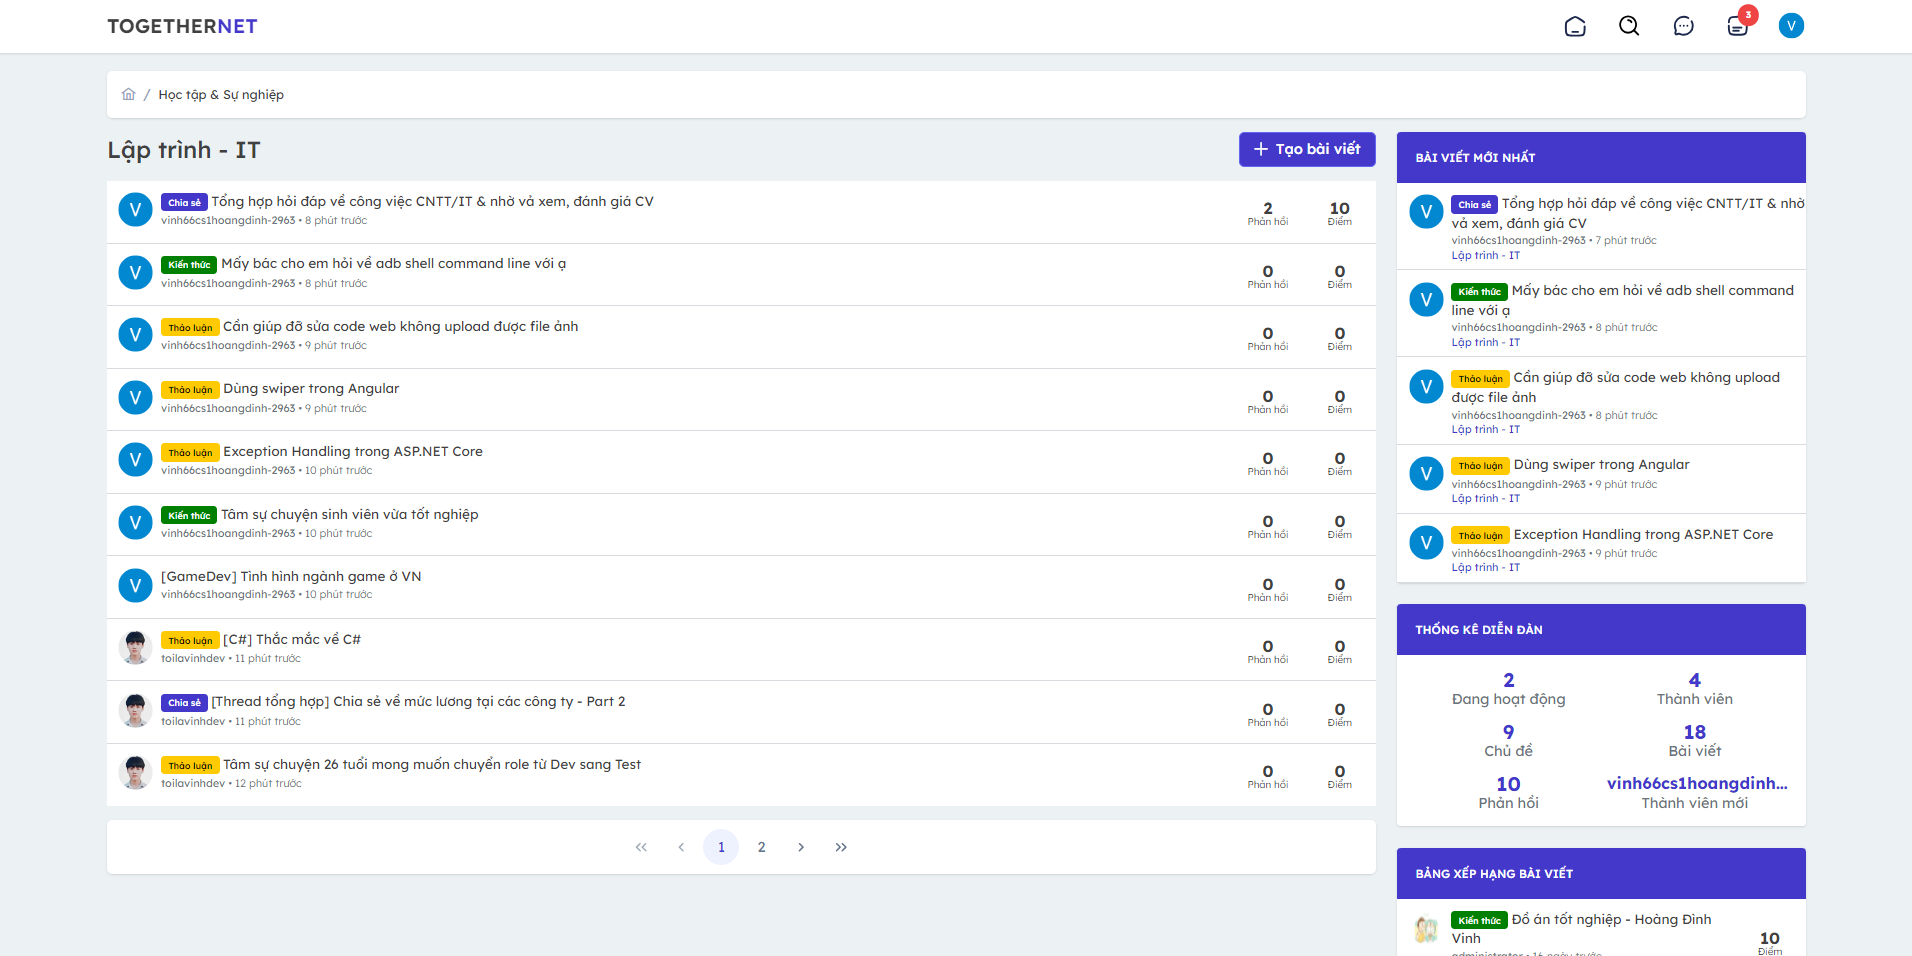
\includegraphics[width=1\linewidth]{figures/demo/topic-page.png}
        \caption{UI Chủ đề}
    \end{figure}
    Màn hình danh sách bài viết trong một chủ đề hiển thị các bài viết với tiêu
    đề, tác giả và thời gian đăng. Người dùng có thể chọn bài viết để đọc bài
    viết cụ thể.

    \subsection{UI Bài viết}
    \begin{figure}[H]
        \centering
        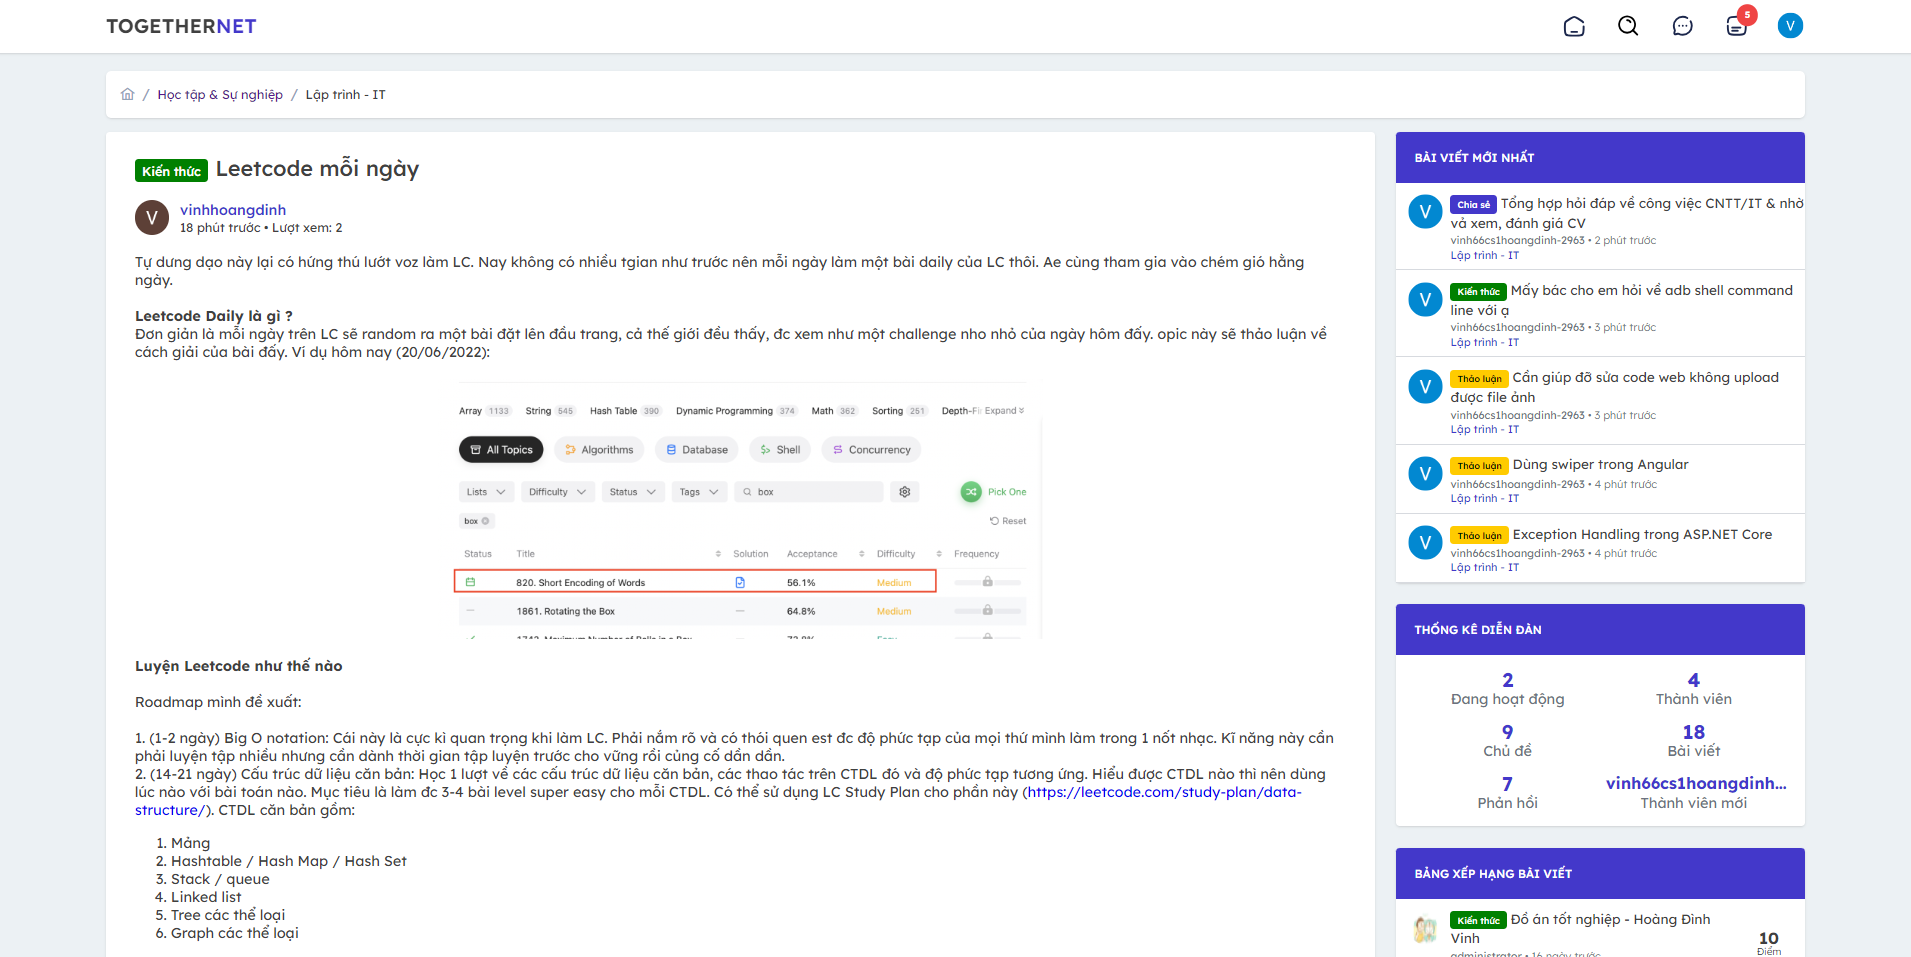
\includegraphics[width=1\linewidth]{figures/demo/post-detail-page.png}
        \caption{UI Bài viết}
    \end{figure}
    Bài viết hiển thị nội dung bài viết bao gồm tiêu đề, nội dung và ảnh. Bên
    cạnh đó, các thông tin bổ sung như tác giả, thời gian đăng và số lượt xem
    cũng được hiển thị đầy đủ, giúp người dùng hiểu hơn về nội dung và chất lượng
    bài viết.

    \subsection{UI Bình luận}
    \begin{figure}[H]
        \centering
        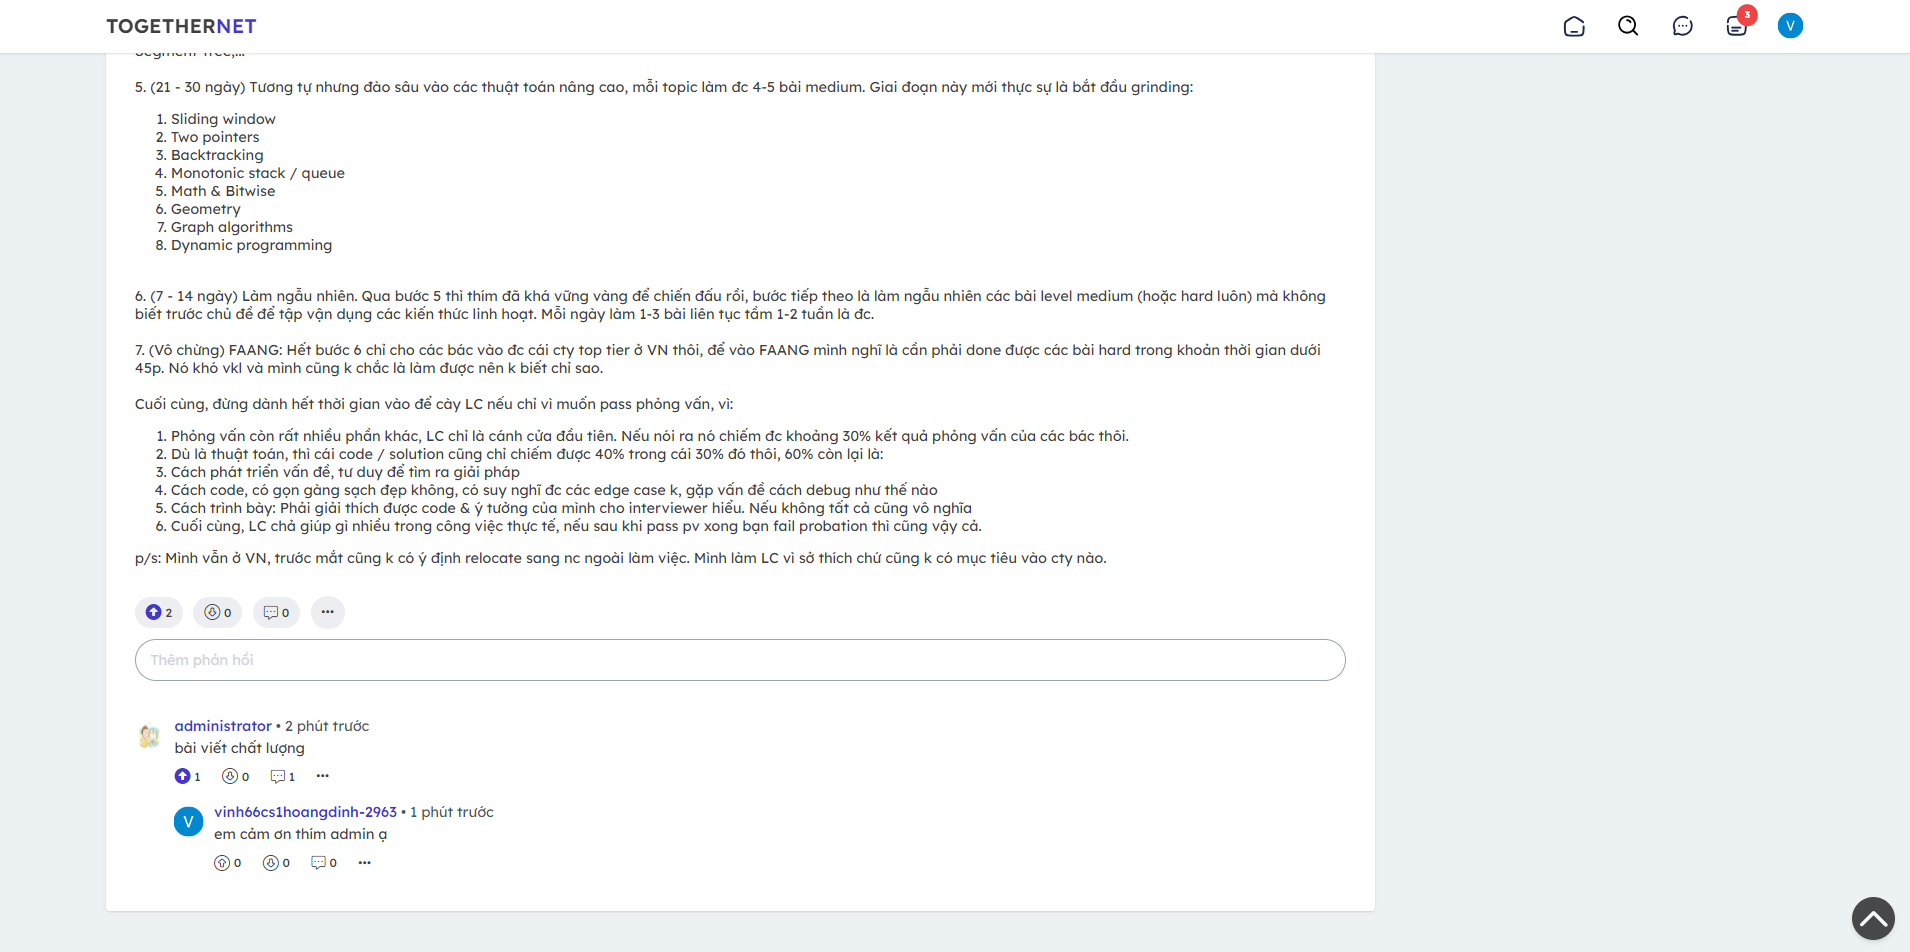
\includegraphics[width=1\linewidth]{figures/demo/post-detail-page-2.png}
        \caption{UI Bình luận}
    \end{figure}
    Người dùng có thể để lại bình luận, xem các phản hồi từ người khác và tham
    gia thảo luận. Ngoài ra, hệ thống vote (bỏ phiếu) giúp đánh giá chất lượng
    các bình luận.

    \subsection{UI Tạo mới bài viết}
    \begin{figure}[H]
        \centering
        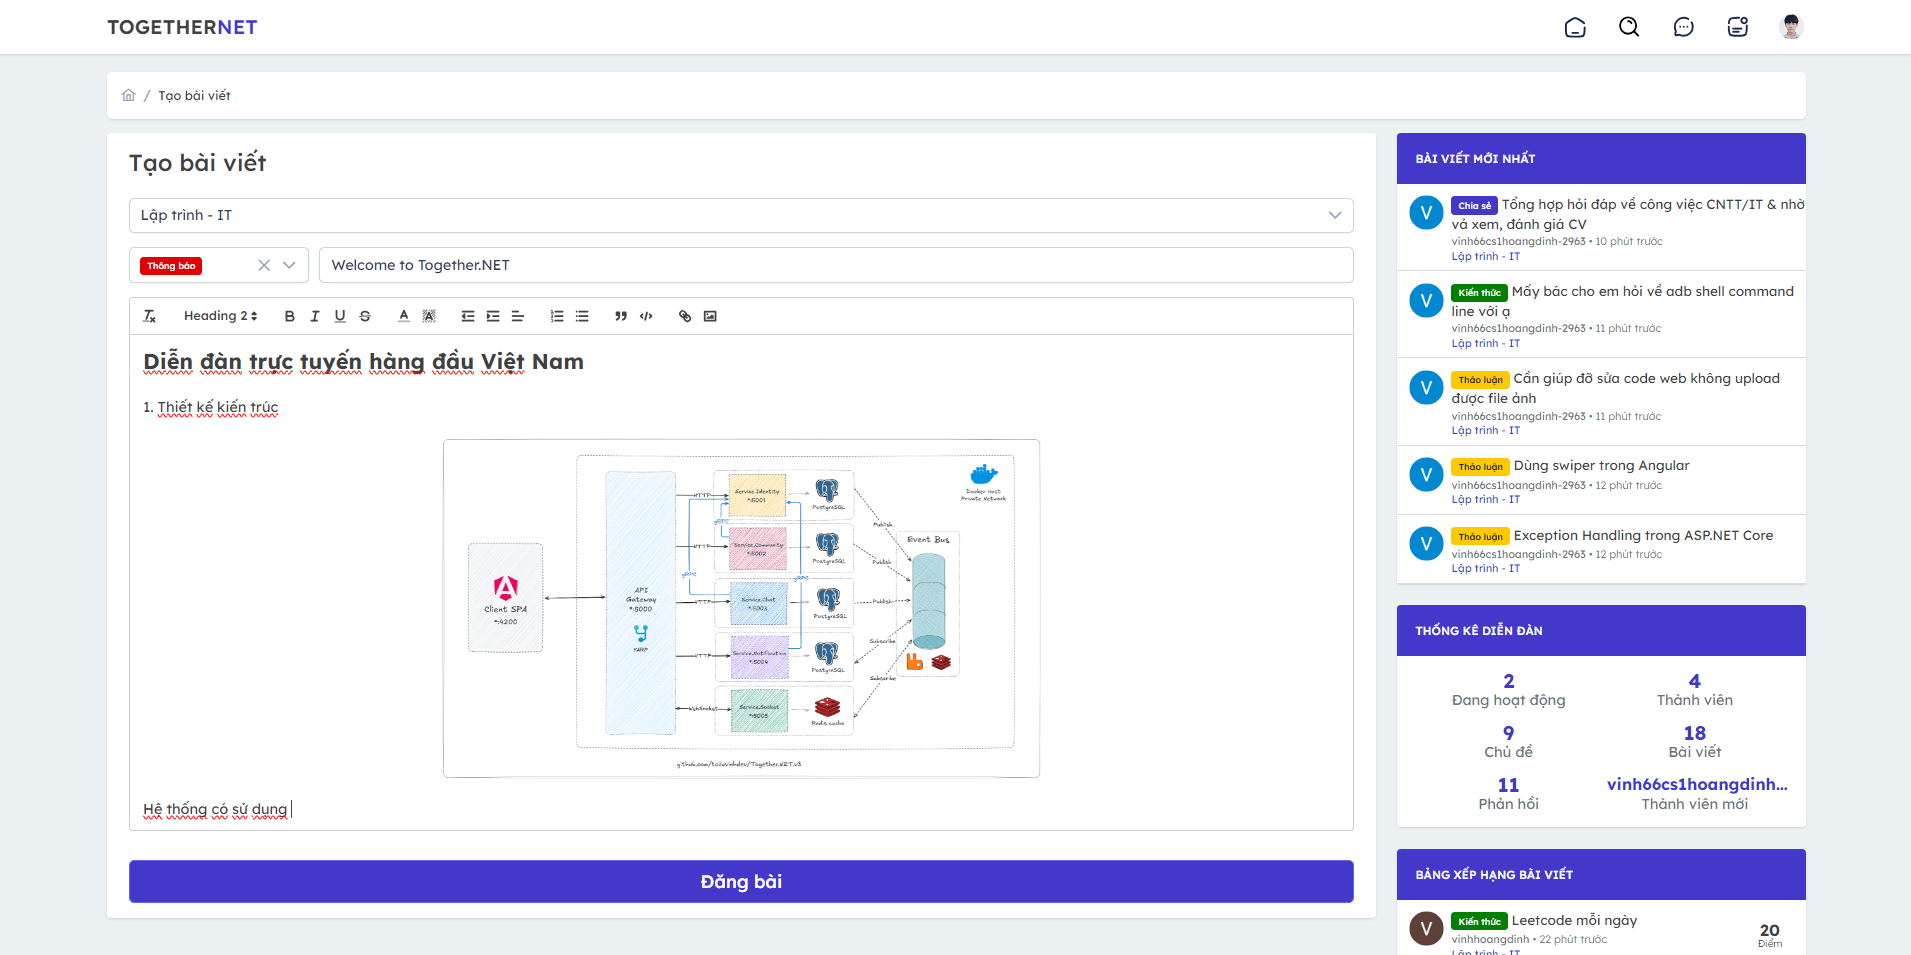
\includegraphics[width=1\linewidth]{figures/demo/create-post-page.png}
        \caption{UI Tạo mới bài viết}
    \end{figure}
    UI này nhằm tạo điều kiện thuận lợi cho người dùng trong việc tạo bài
    viết, chia sẻ ý tưởng và thông tin một cách trực quan và hiệu quả.

    \subsection{UI Cập nhật bài viết}
    \begin{figure}[H]
        \centering
        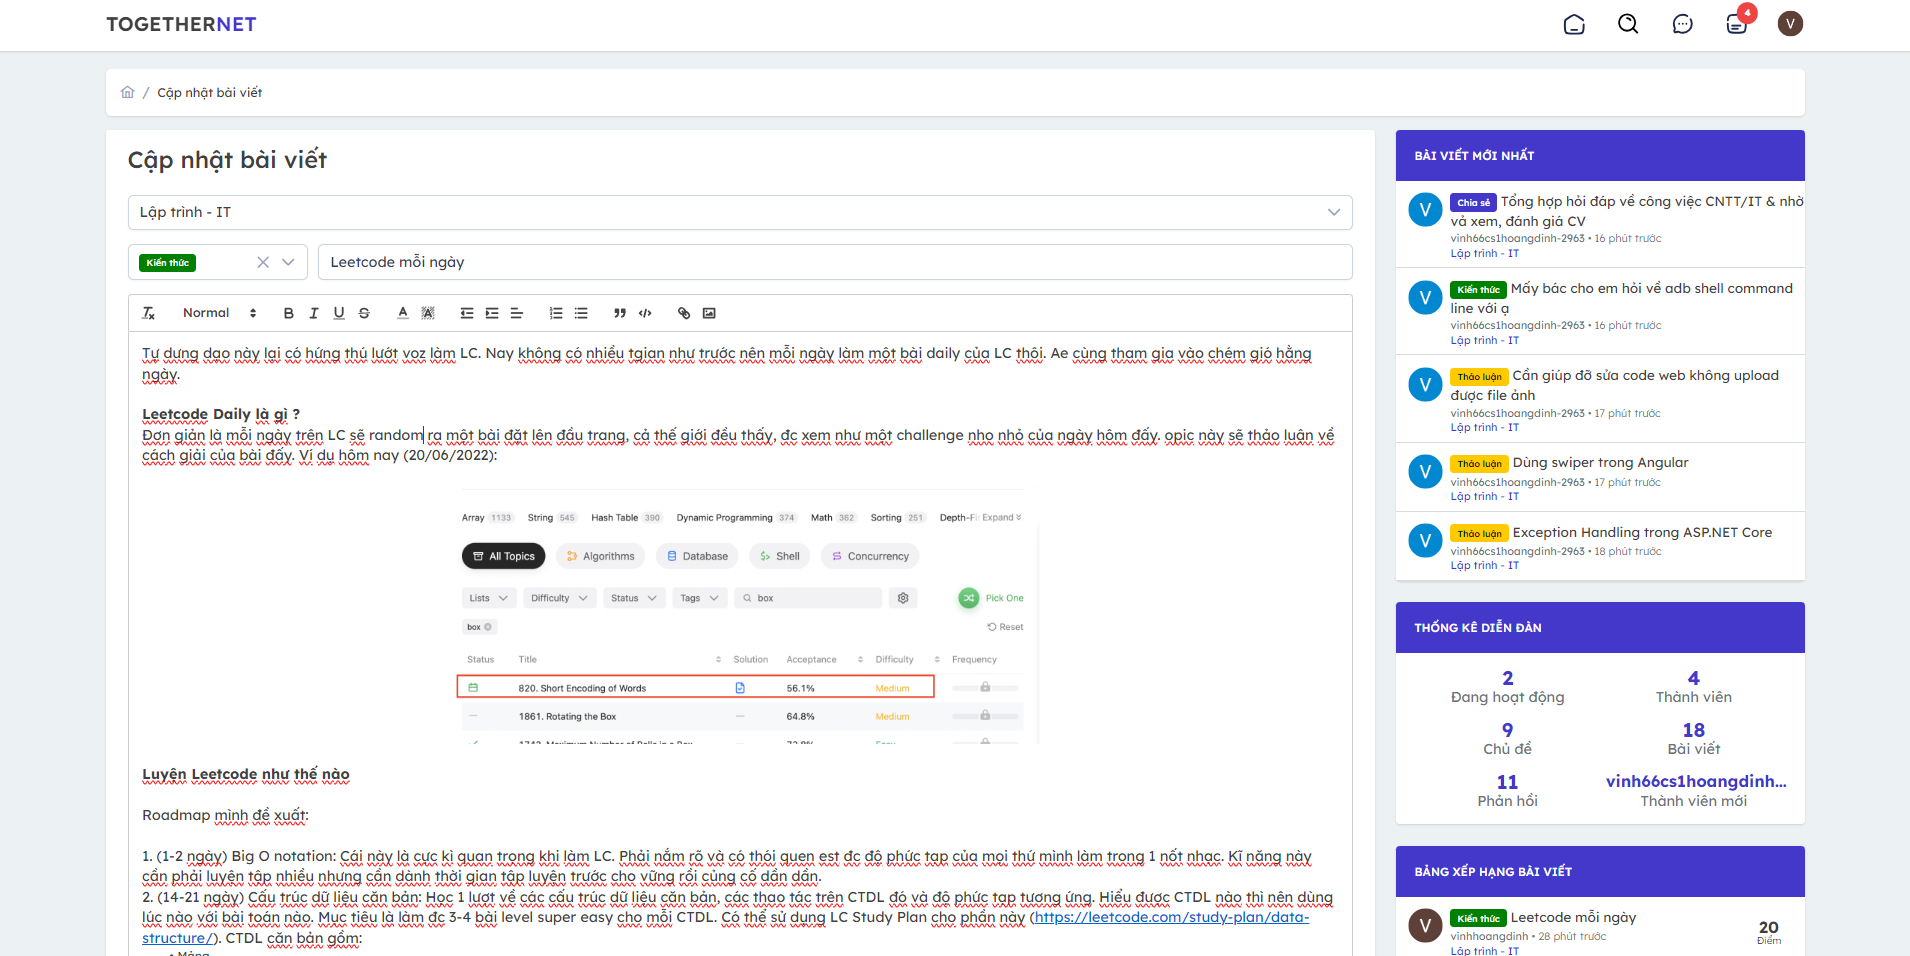
\includegraphics[width=1\linewidth]{figures/demo/update-post-page.png}
        \caption{UI Cập nhật bài viết}
    \end{figure}
    Người dùng dễ dàng chỉnh sửa nội dung, thêm hình ảnh, định dạng văn bản và lưu
    thay đổi, đảm bảo nội dung luôn mới mẻ và chính xác.

    \subsection{UI Trang cá nhân thành viên}
    \begin{figure}[H]
        \centering
        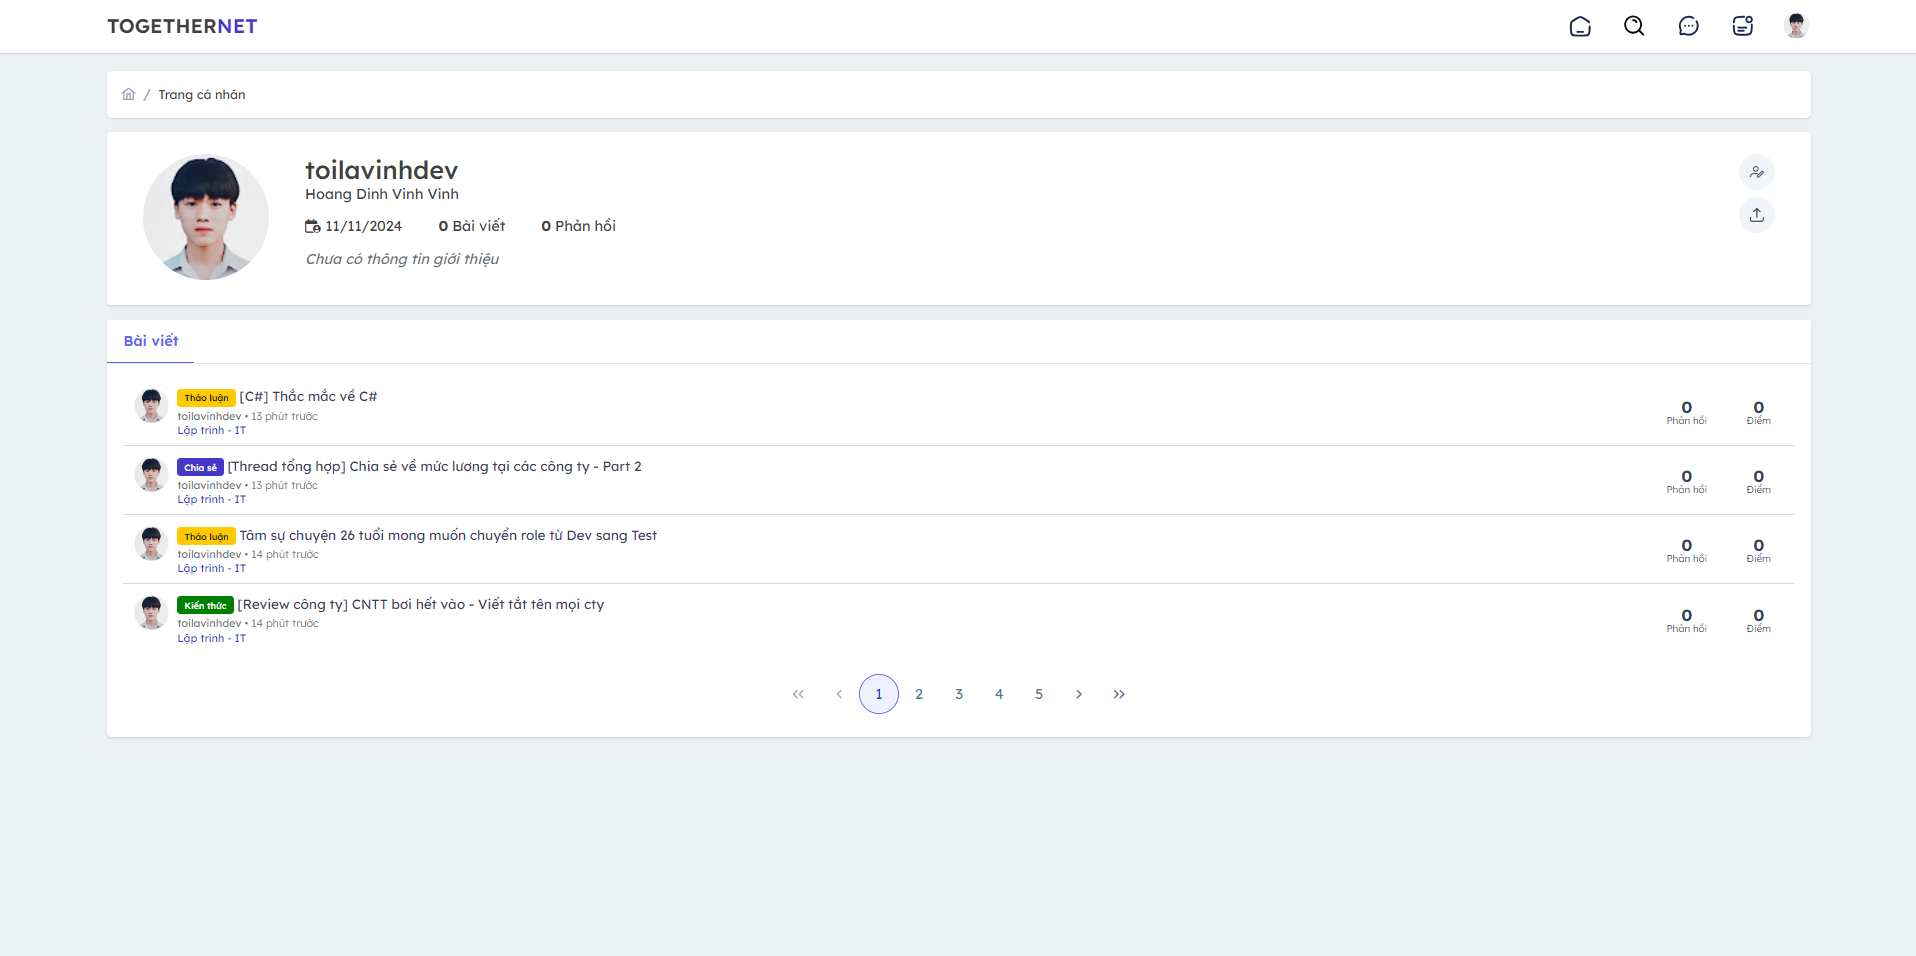
\includegraphics[width=1\linewidth]{figures/demo/profile-page.png}
        \caption{UI Trang cá nhân thành viên}
    \end{figure}

    \subsection{UI Cập nhật thông tin}
    \begin{figure}[H]
        \centering
        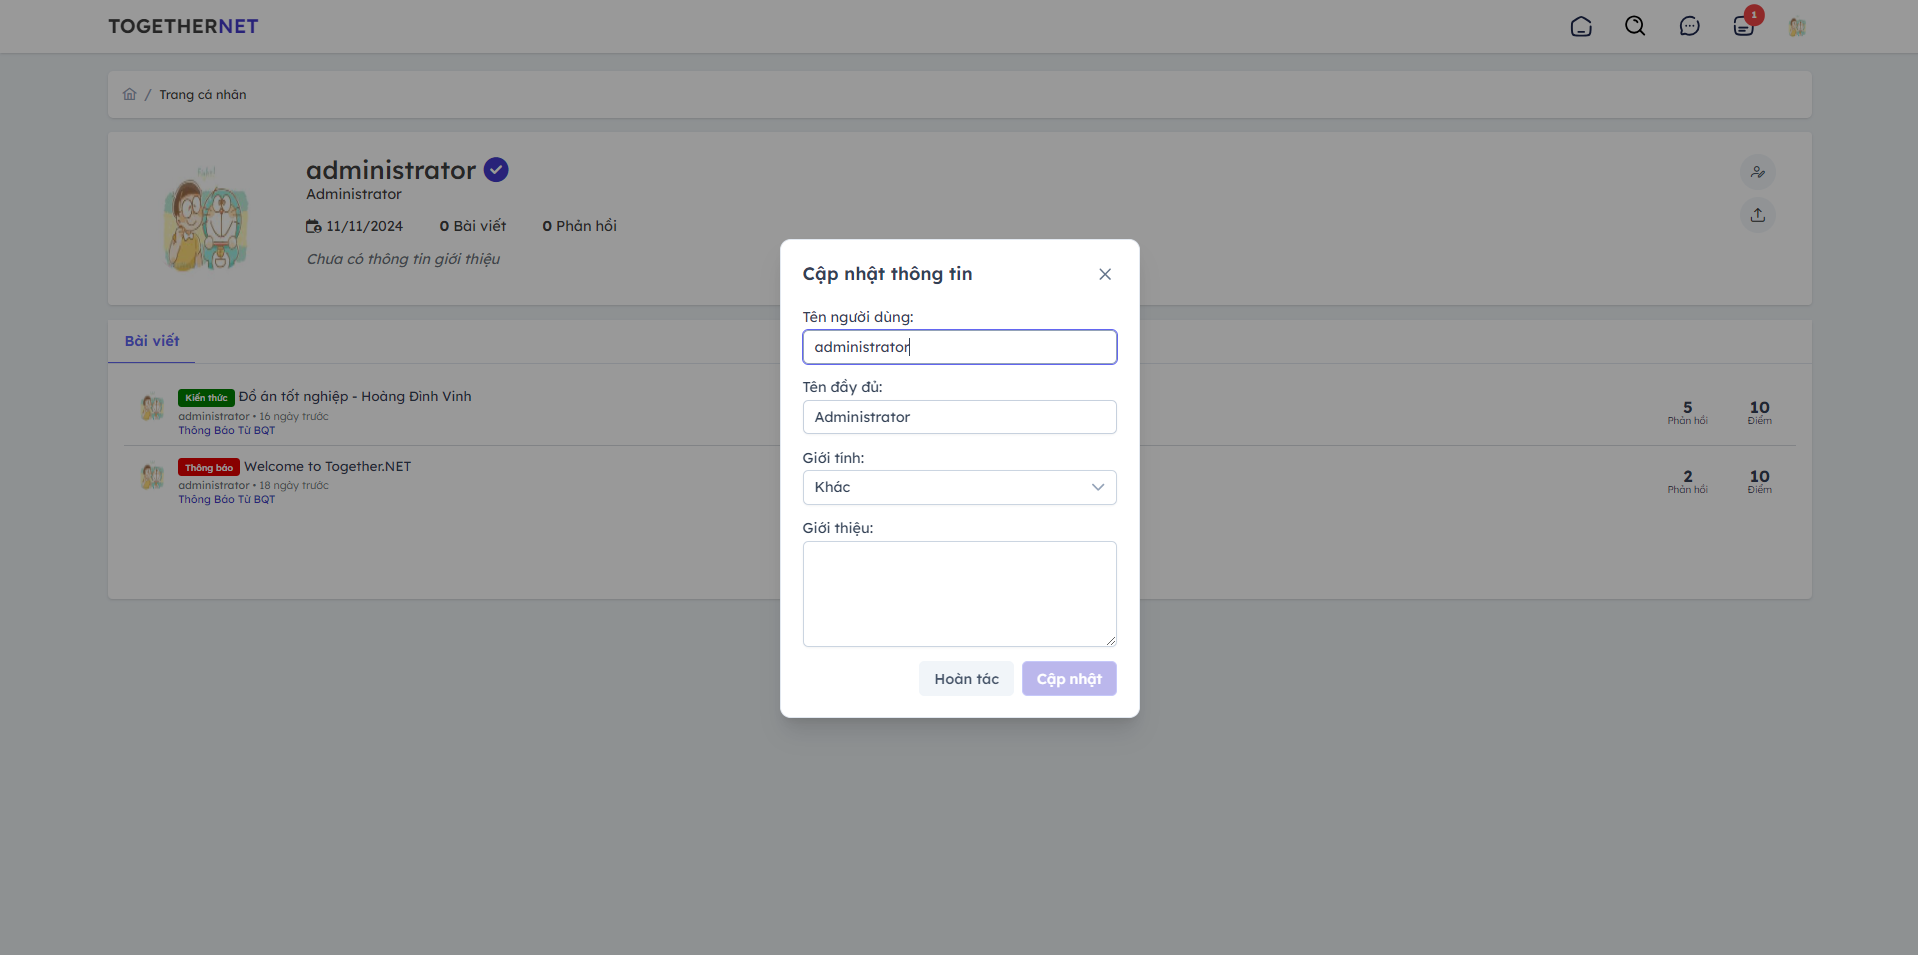
\includegraphics[width=1\linewidth]{
            figures/demo/update-profile-page.png
        }
        \caption{UI Cập nhật thông tin}
    \end{figure}

    \subsection{UI Cài đặt tài khoản}
    \begin{figure}[H]
        \centering
        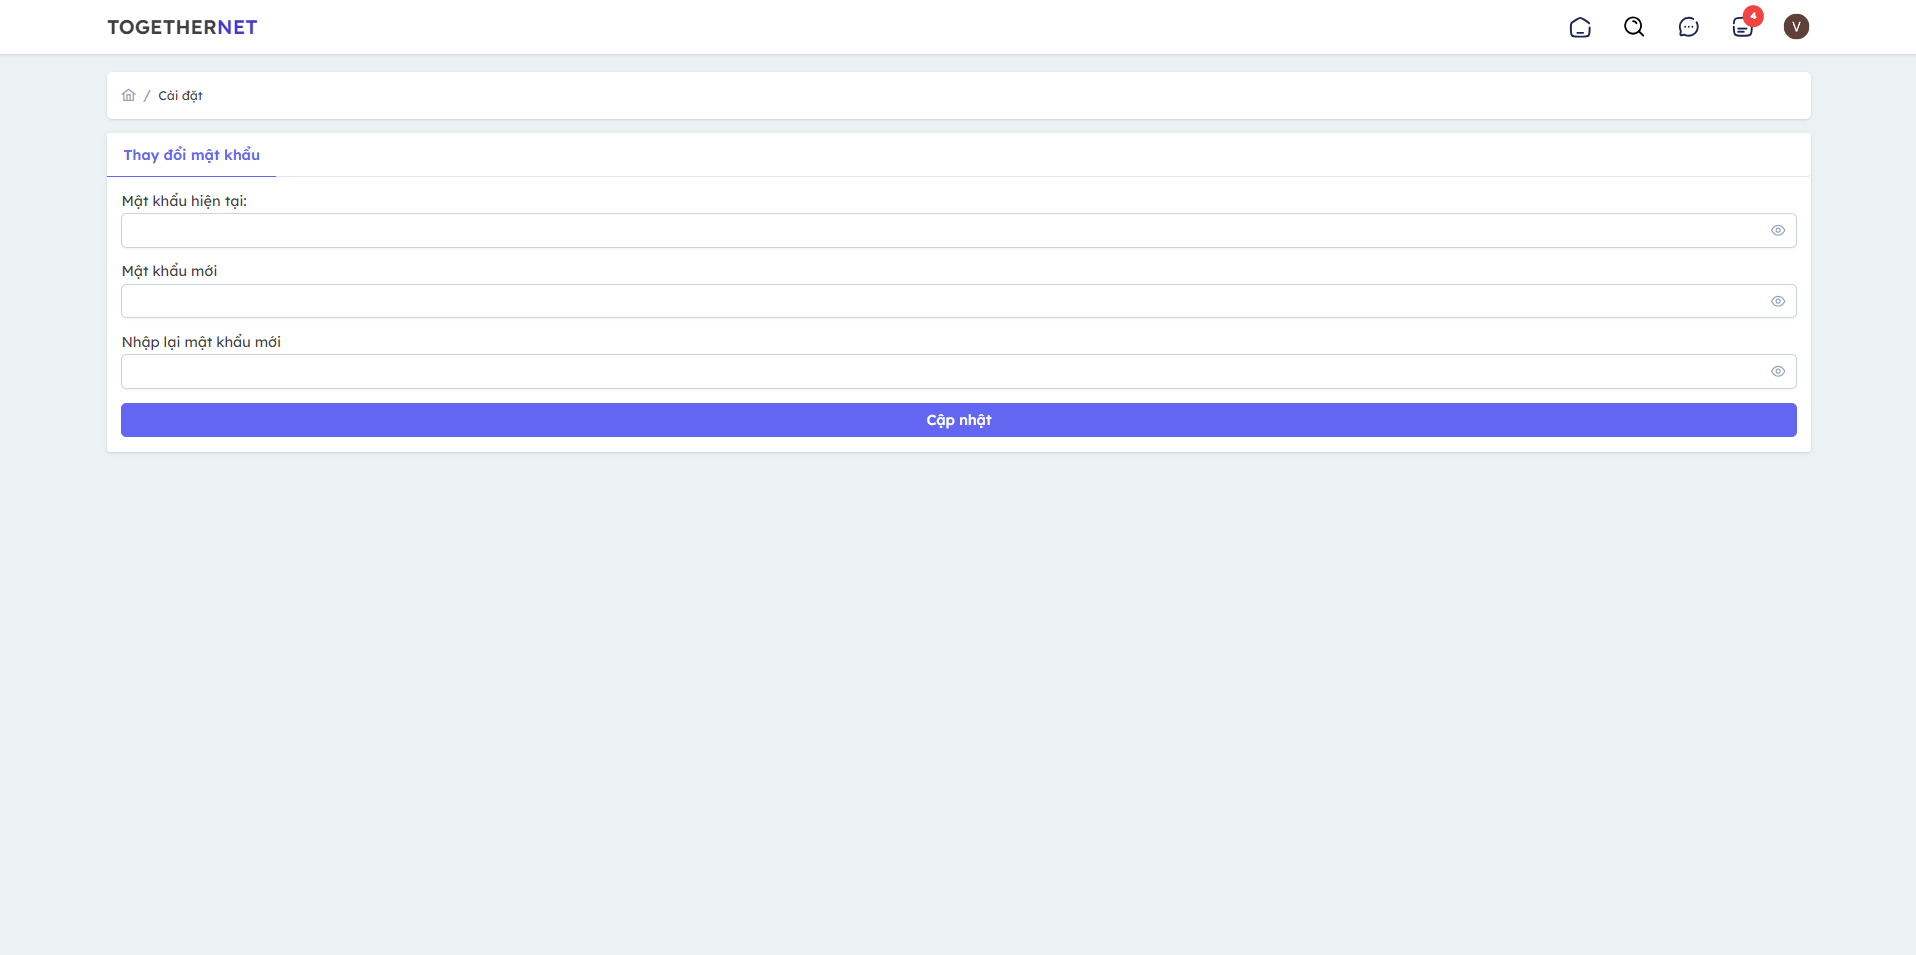
\includegraphics[width=1\linewidth]{
            figures/demo/account-setting-page.png
        }
        \caption{UI Cài đặt tài khoản}
    \end{figure}

    \subsection{UI Tìm kiếm}
    \begin{figure}[H]
        \centering
        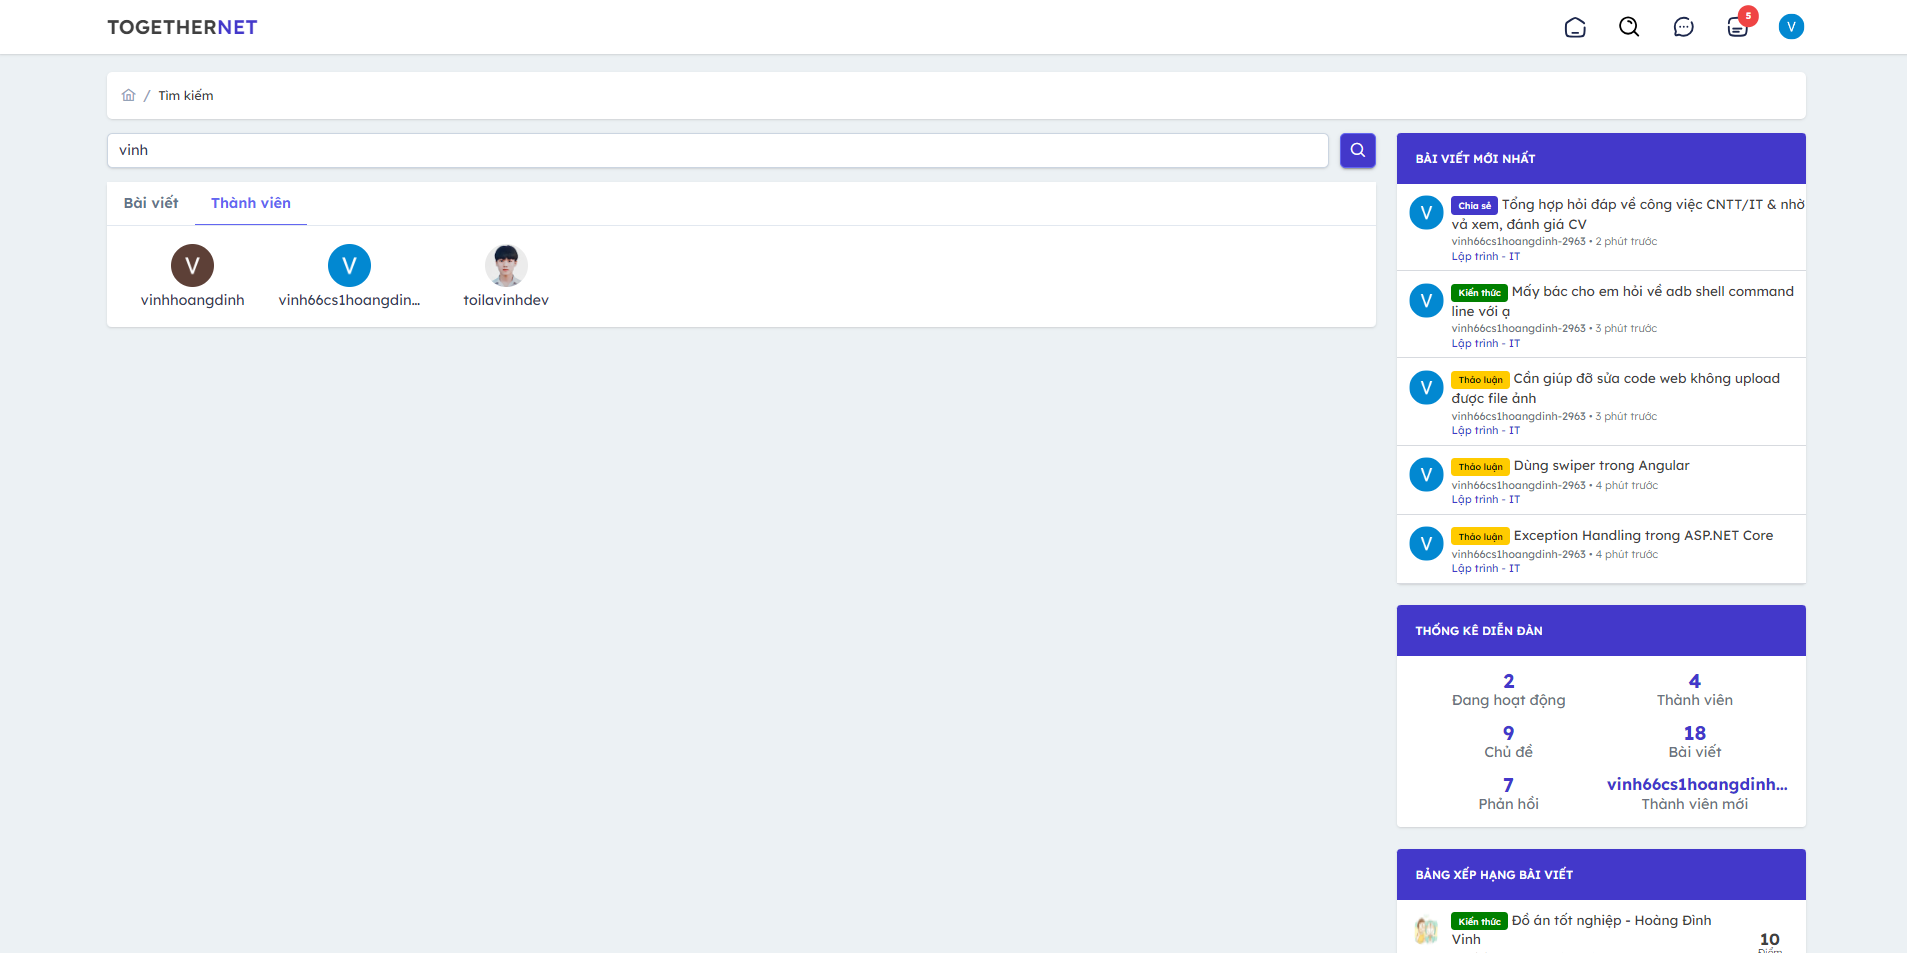
\includegraphics[width=1\linewidth]{figures/demo/search-page.png}
        \caption{UI Tìm kiếm}
    \end{figure}

    \subsection{UI Thông báo}
    \begin{figure}[H]
        \centering
        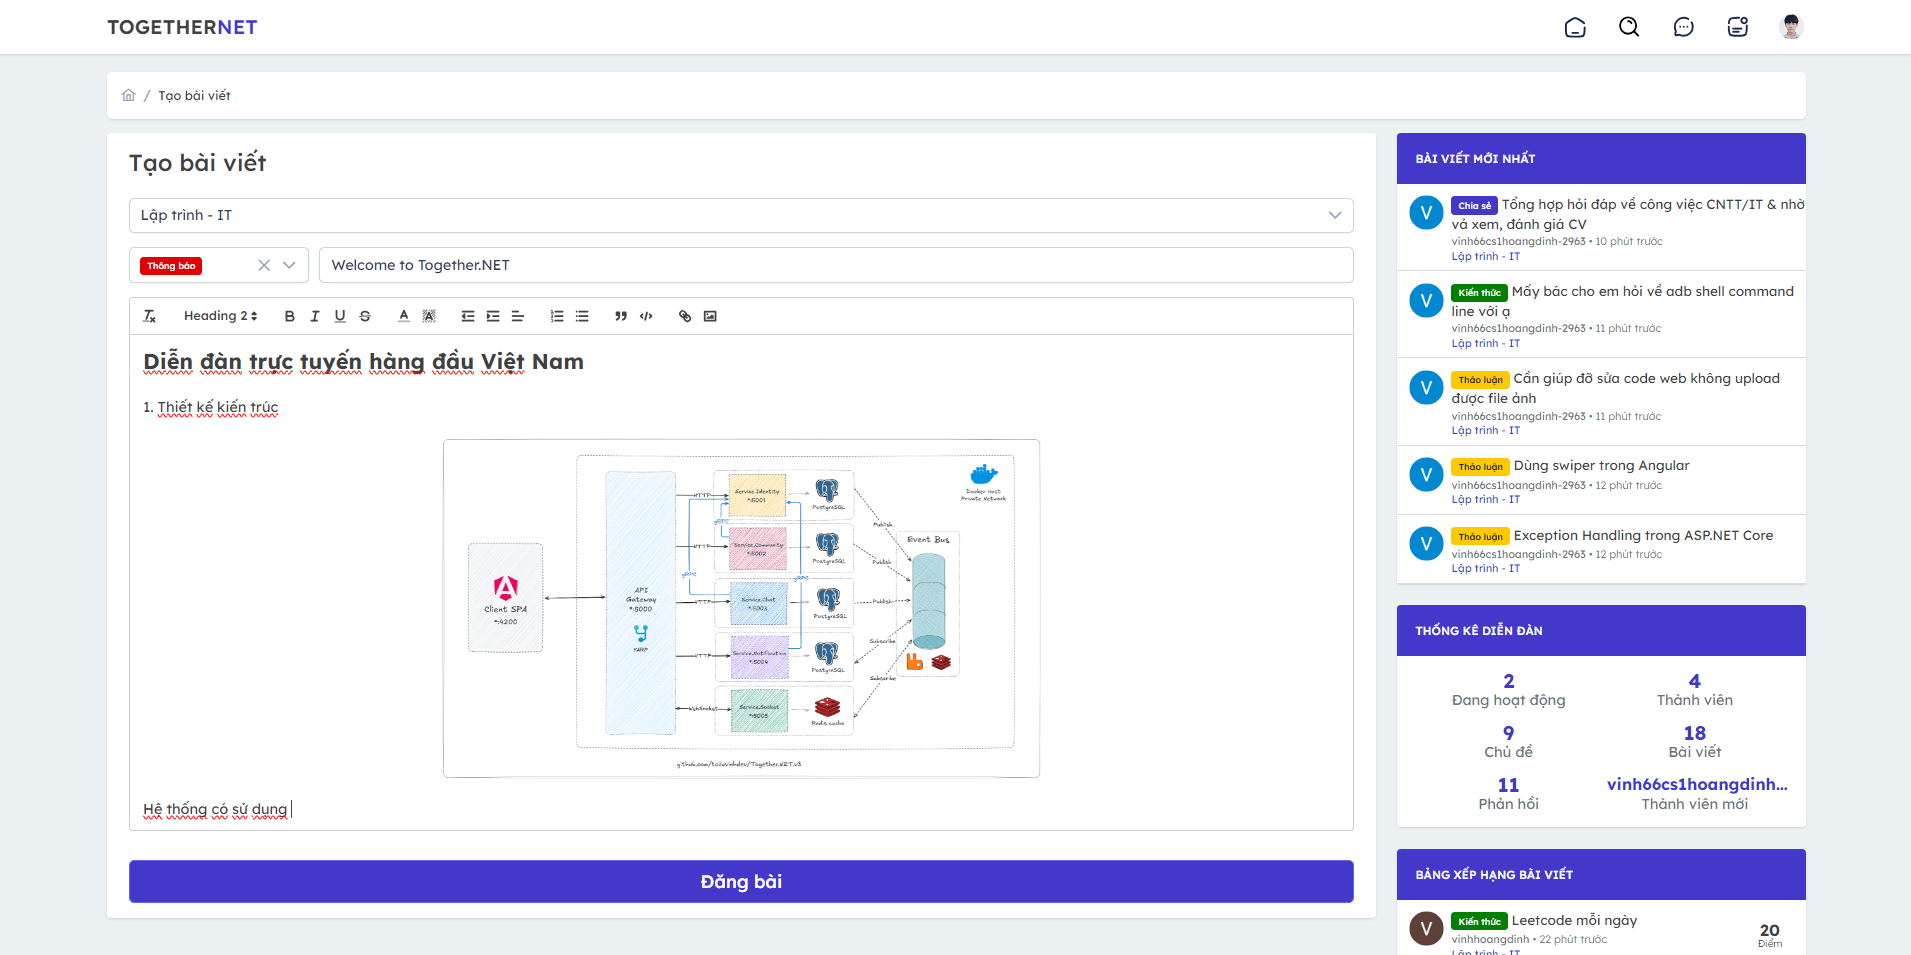
\includegraphics[width=1\linewidth]{figures/demo/create-post-page.png}
        \caption{UI Thông báo}
    \end{figure}

    \subsection{UI Chat}
    \begin{figure}[H]
        \centering
        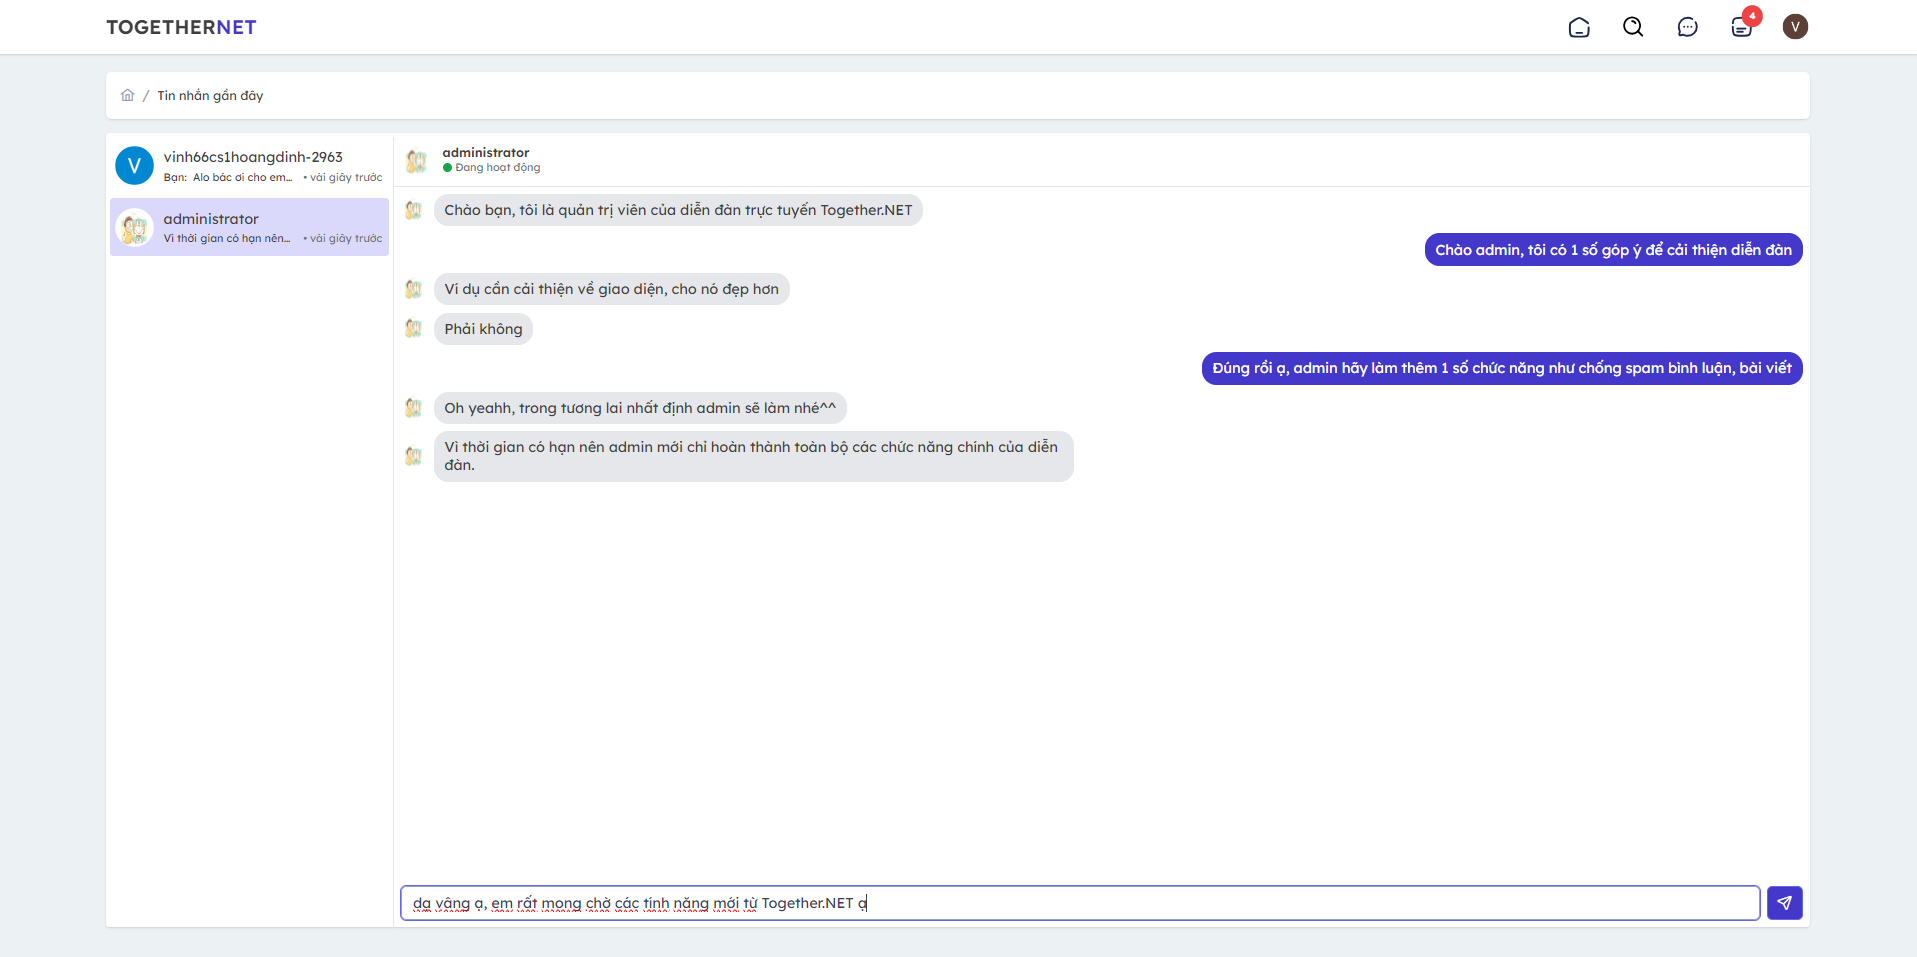
\includegraphics[width=1\linewidth]{figures/demo/chat-page.png}
        \caption{UI Chat}
    \end{figure}

    \subsection{UI Thống kê diễn đàn}
    \begin{figure}[H]
        \centering
        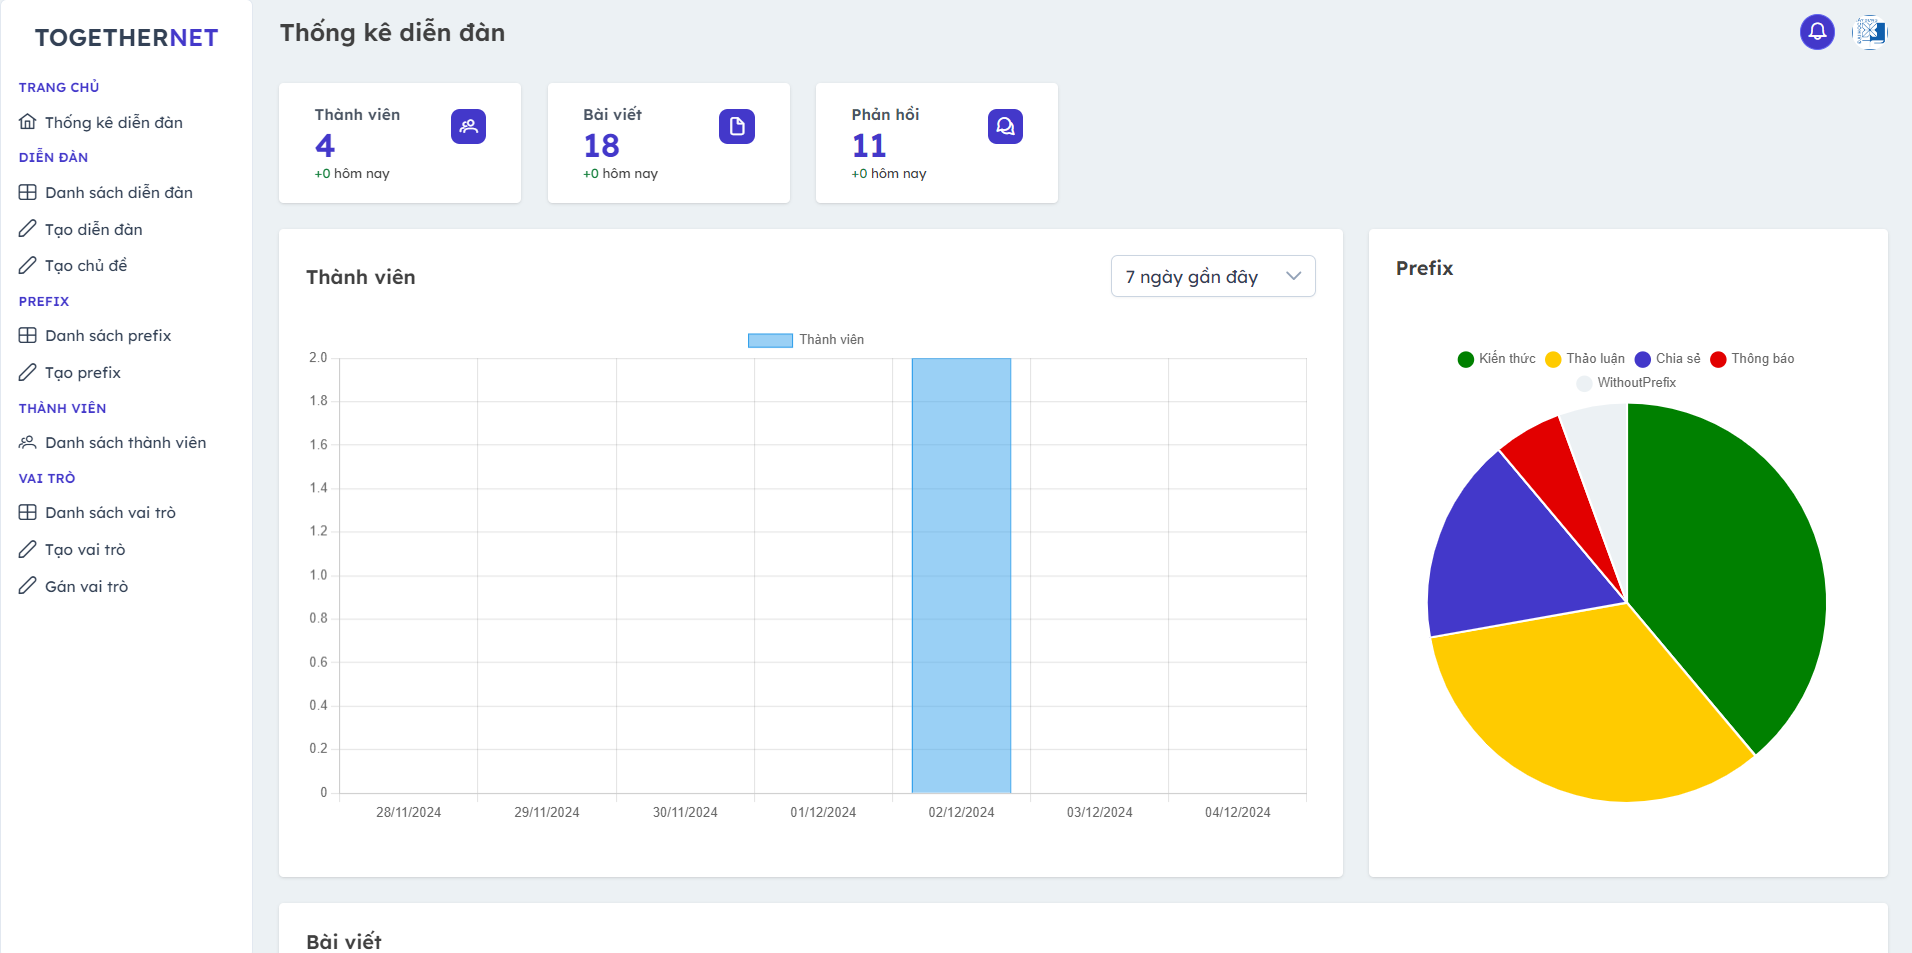
\includegraphics[width=1\linewidth]{figures/demo/management-dashboard-page.png}
        \caption{UI Thống kê diễn đàn}
    \end{figure}

    \subsection{UI Thống kê diễn đàn}
    \begin{figure}[H]
        \centering
        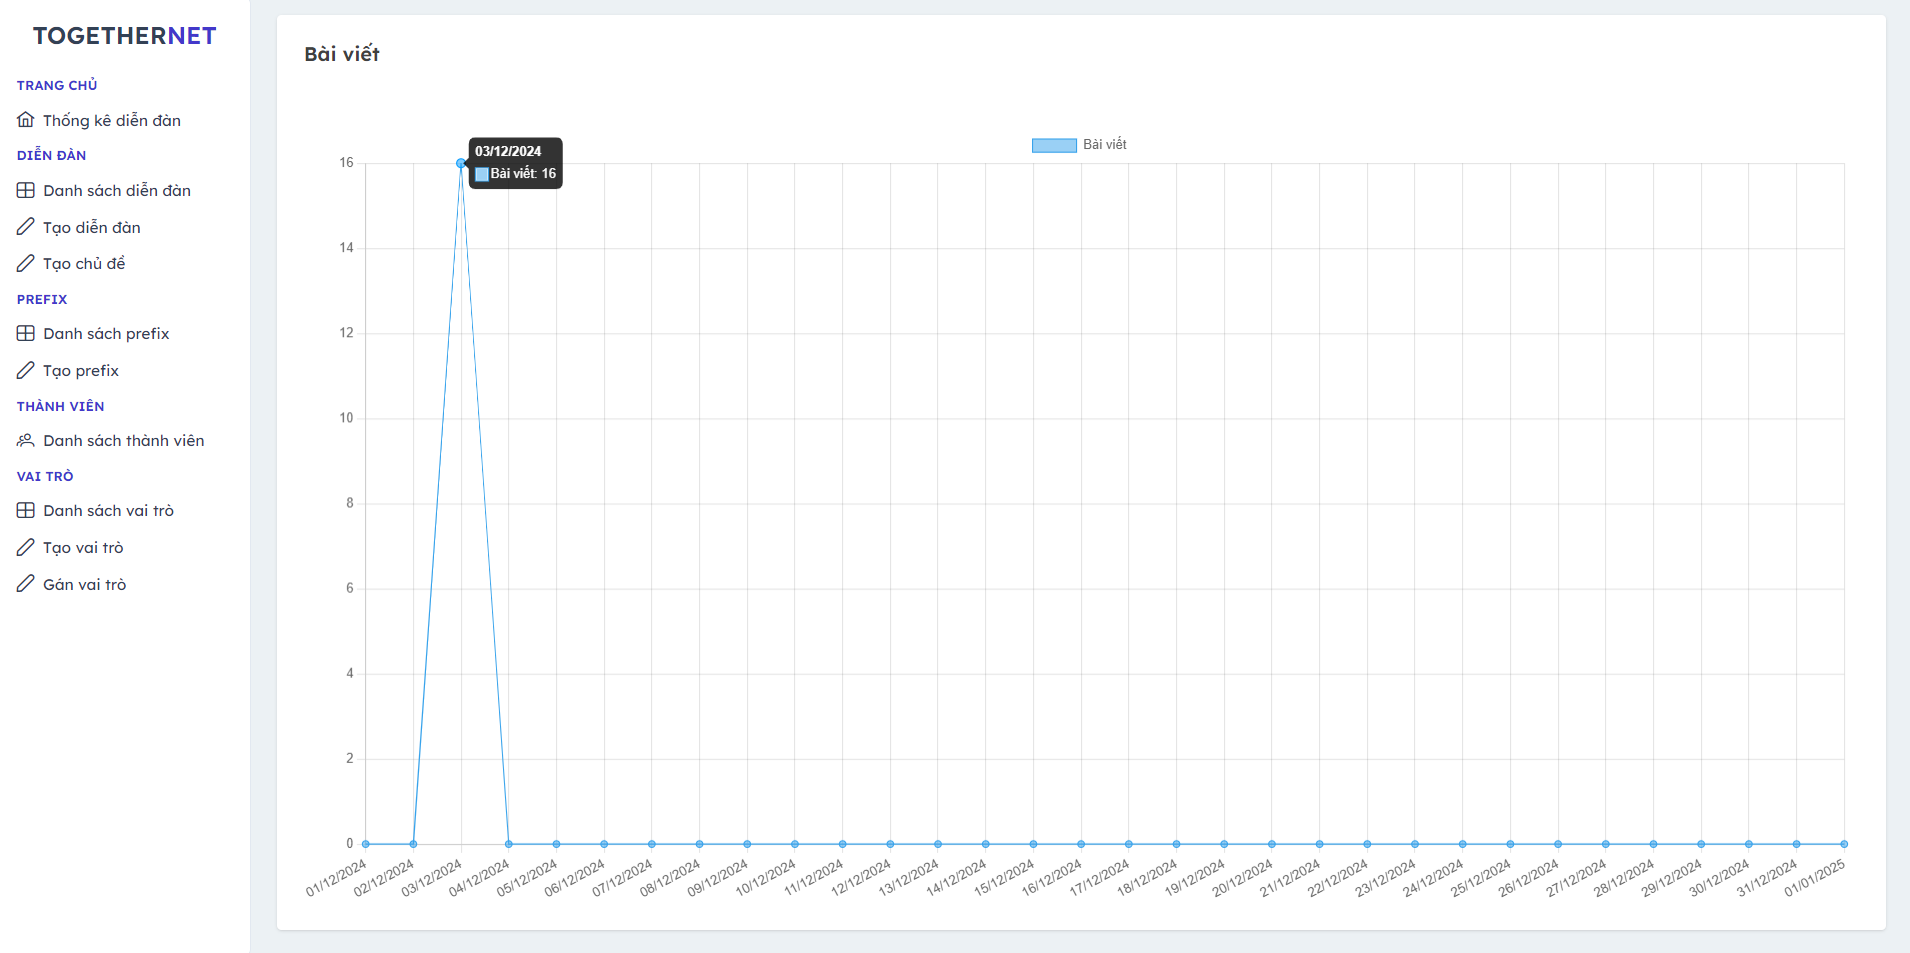
\includegraphics[width=1\linewidth]{figures/demo/management-dashboard-page-2.png}
        \caption{UI Thống kê diễn đàn}
    \end{figure}

    \subsection{UI Danh sách chủ đề}
    \begin{figure}[H]
        \centering
        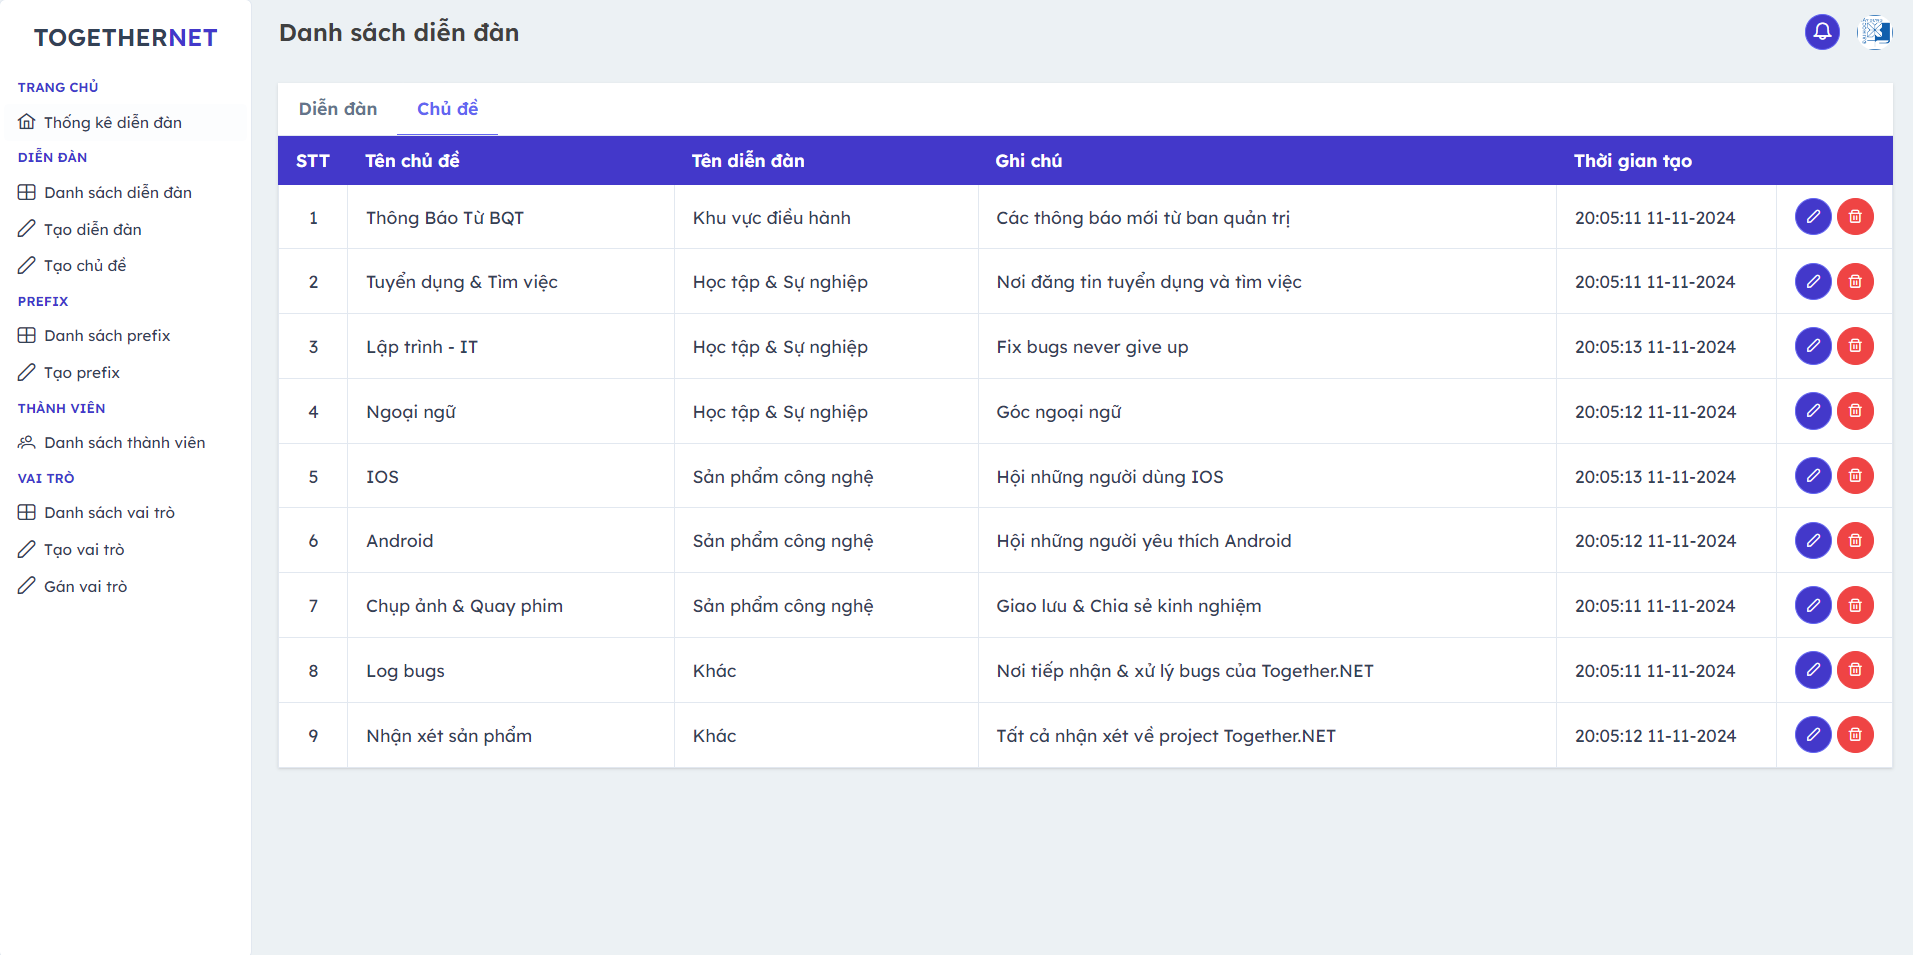
\includegraphics[width=1\linewidth]{figures/demo/management-topic-page.png}
        \caption{UI Danh sách chủ đề}
    \end{figure}

    \subsection{UI Tạo chủ đề}
    \begin{figure}[H]
        \centering
        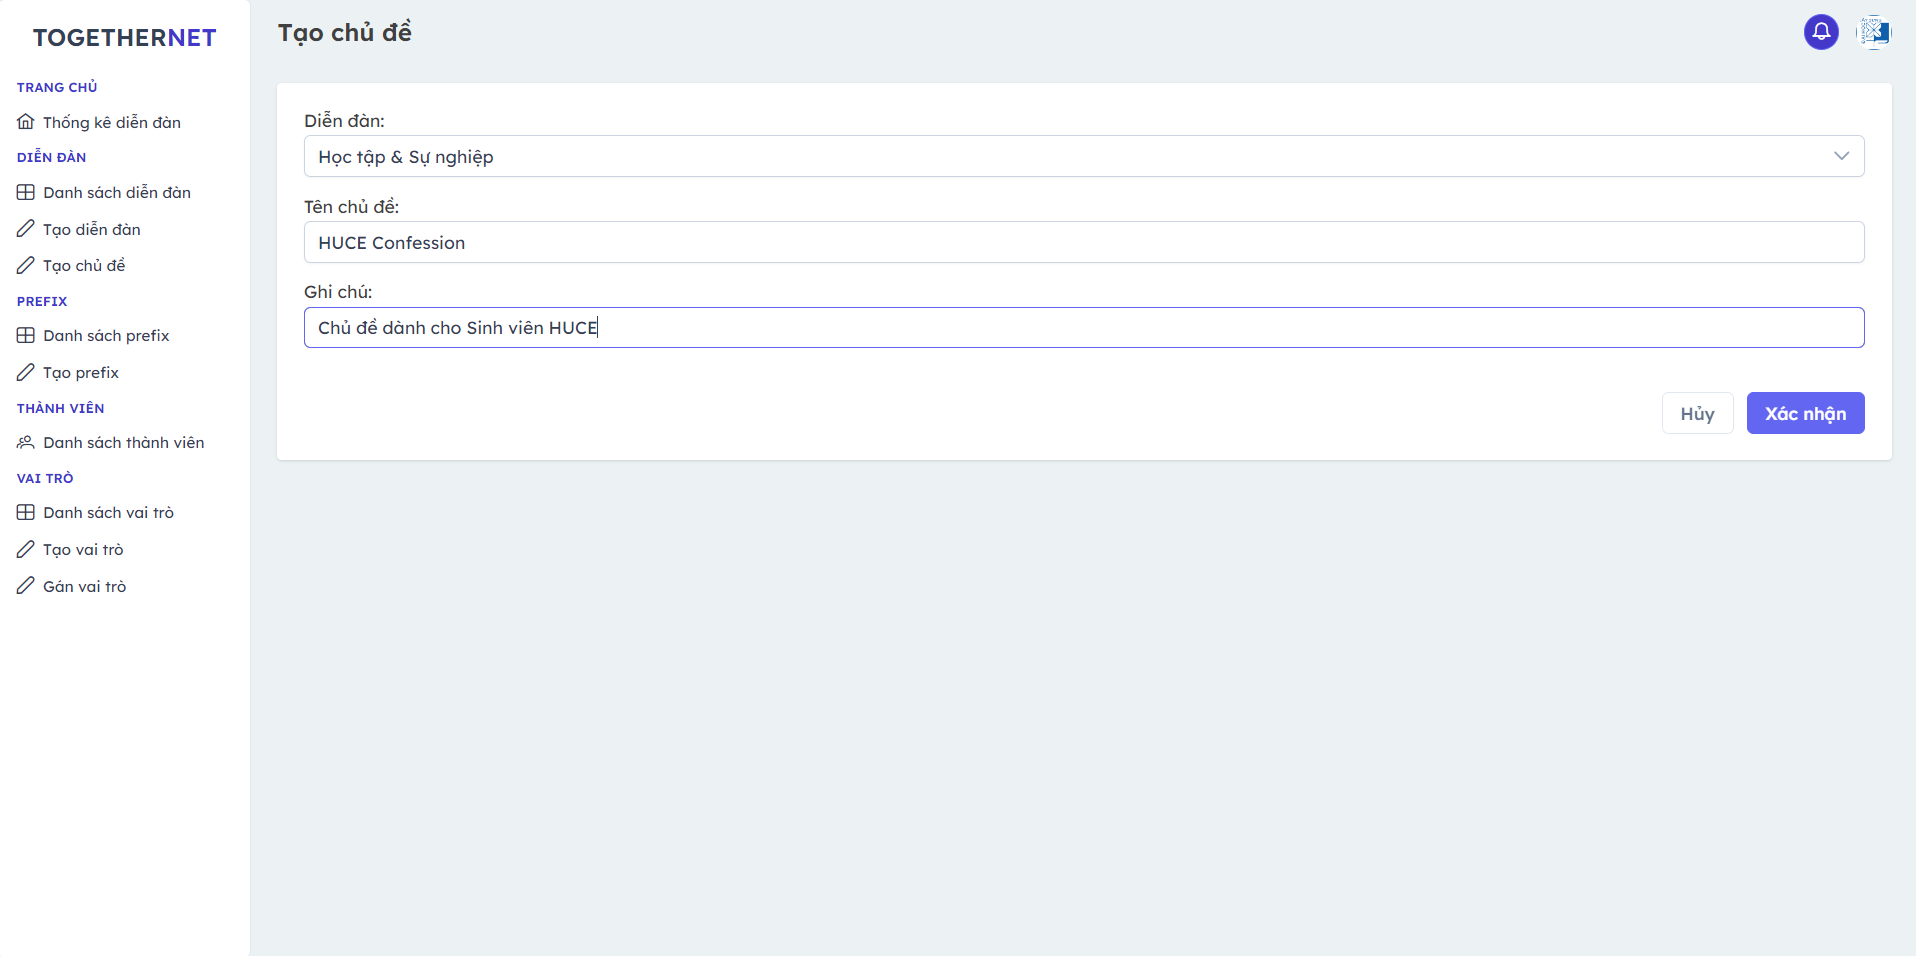
\includegraphics[width=1\linewidth]{figures/demo/management-topic-create-page.png}
        \caption{UI Tạo chủ đề}
    \end{figure}

    \subsection{UI Tạo chủ đề}
    \begin{figure}[H]
        \centering
        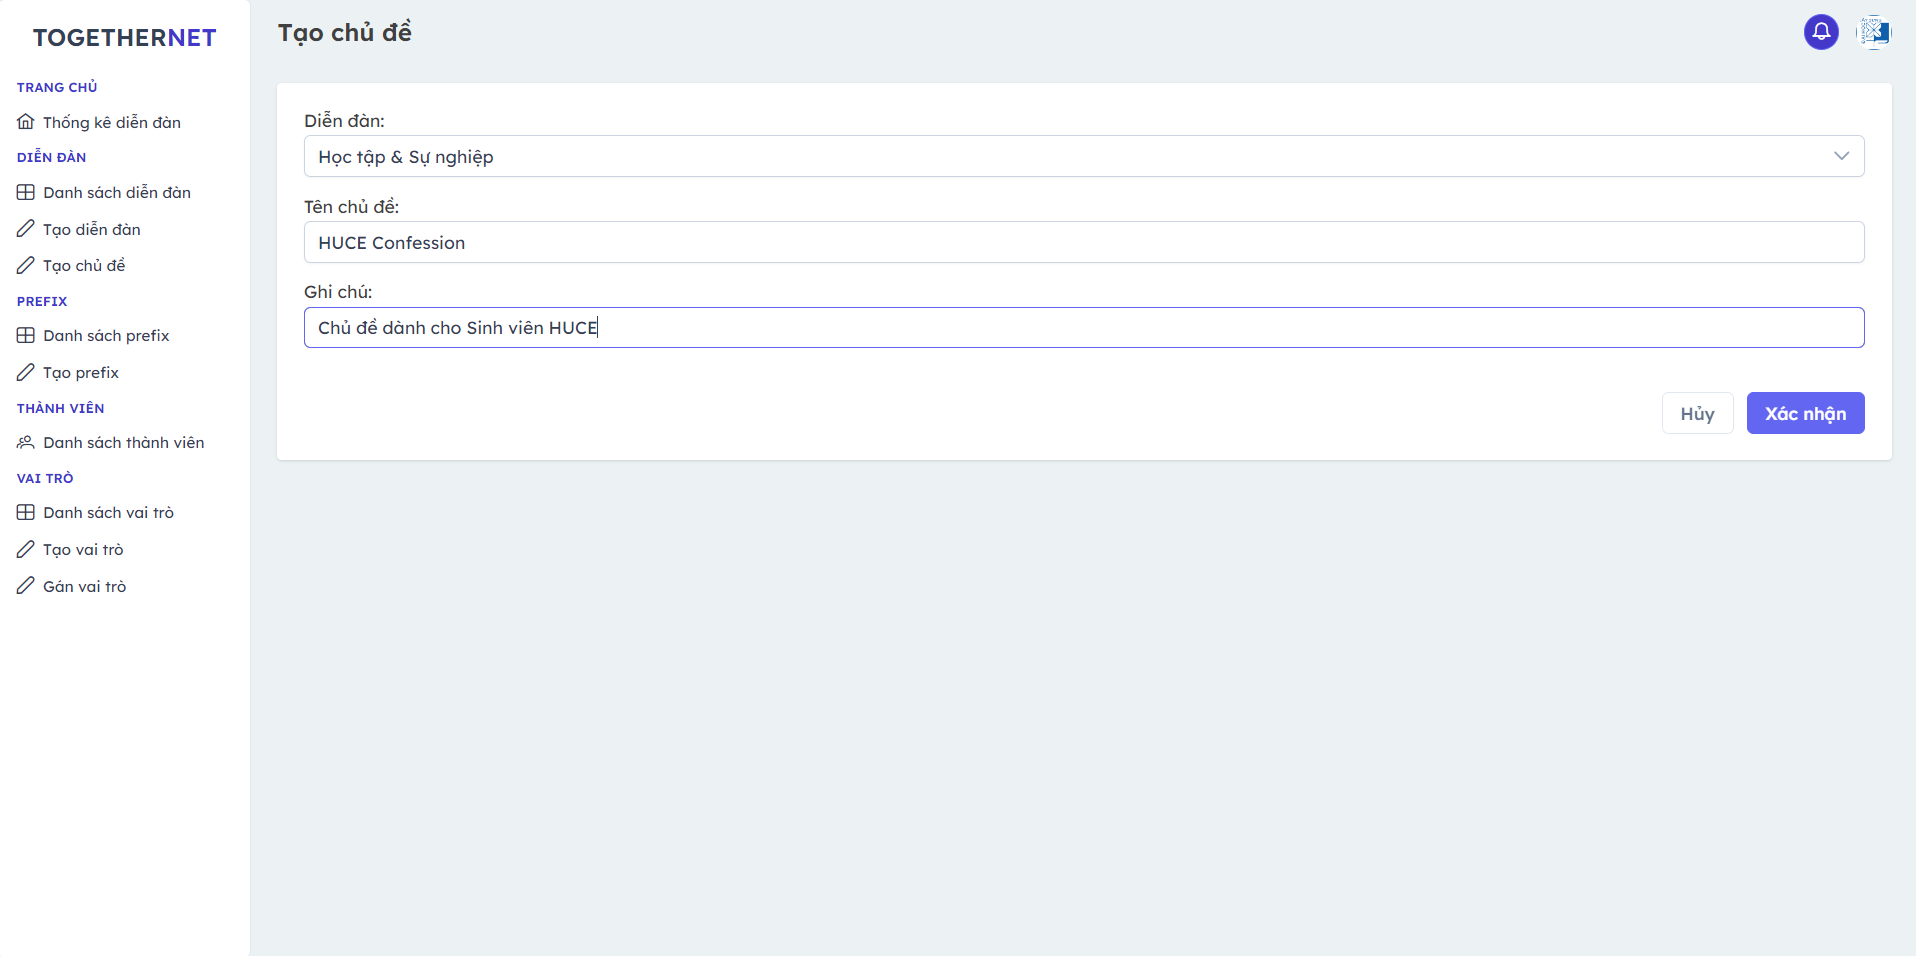
\includegraphics[width=1\linewidth]{figures/demo/management-topic-create-page.png}
        \caption{UI Tạo chủ đề}
    \end{figure}

    \subsection{UI Cập nhật prefix}
    \begin{figure}[H]
        \centering
        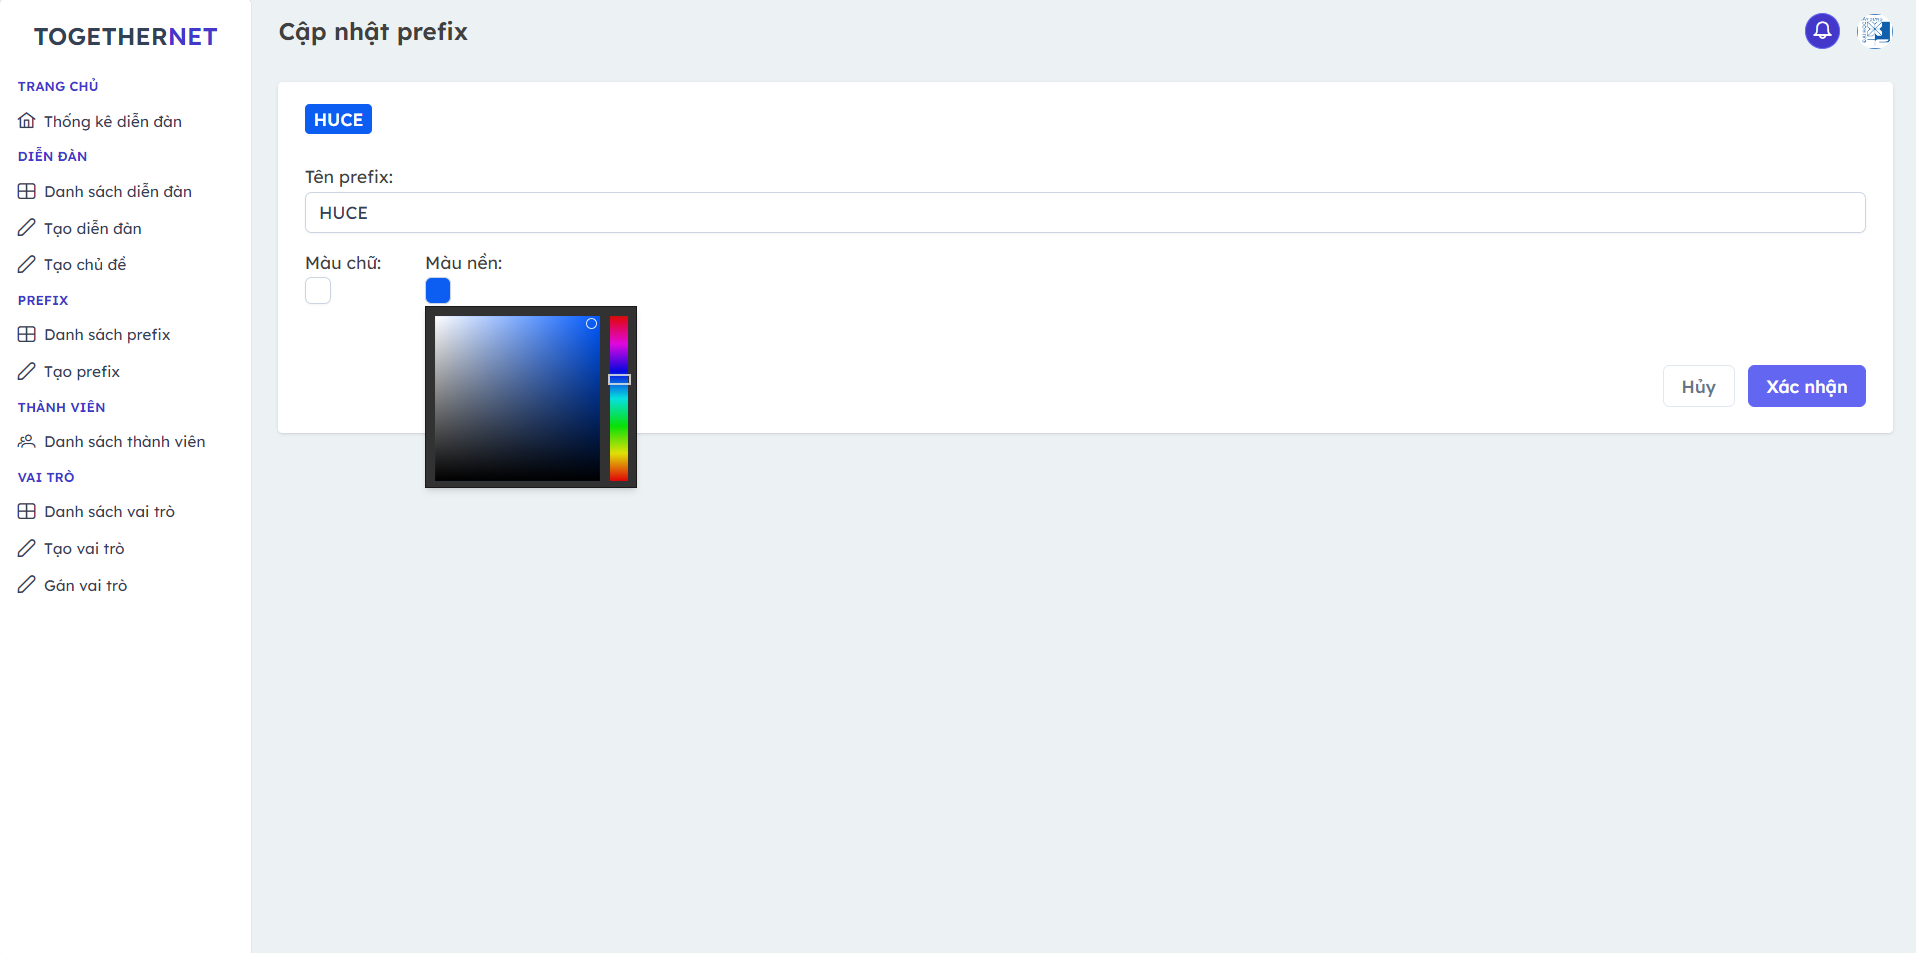
\includegraphics[width=1\linewidth]{figures/demo/management-prefix-create-page.png}
        \caption{UI Cập nhật prefix}
    \end{figure}

    \subsection{UI Danh sách thành viên}
    \begin{figure}[H]
        \centering
        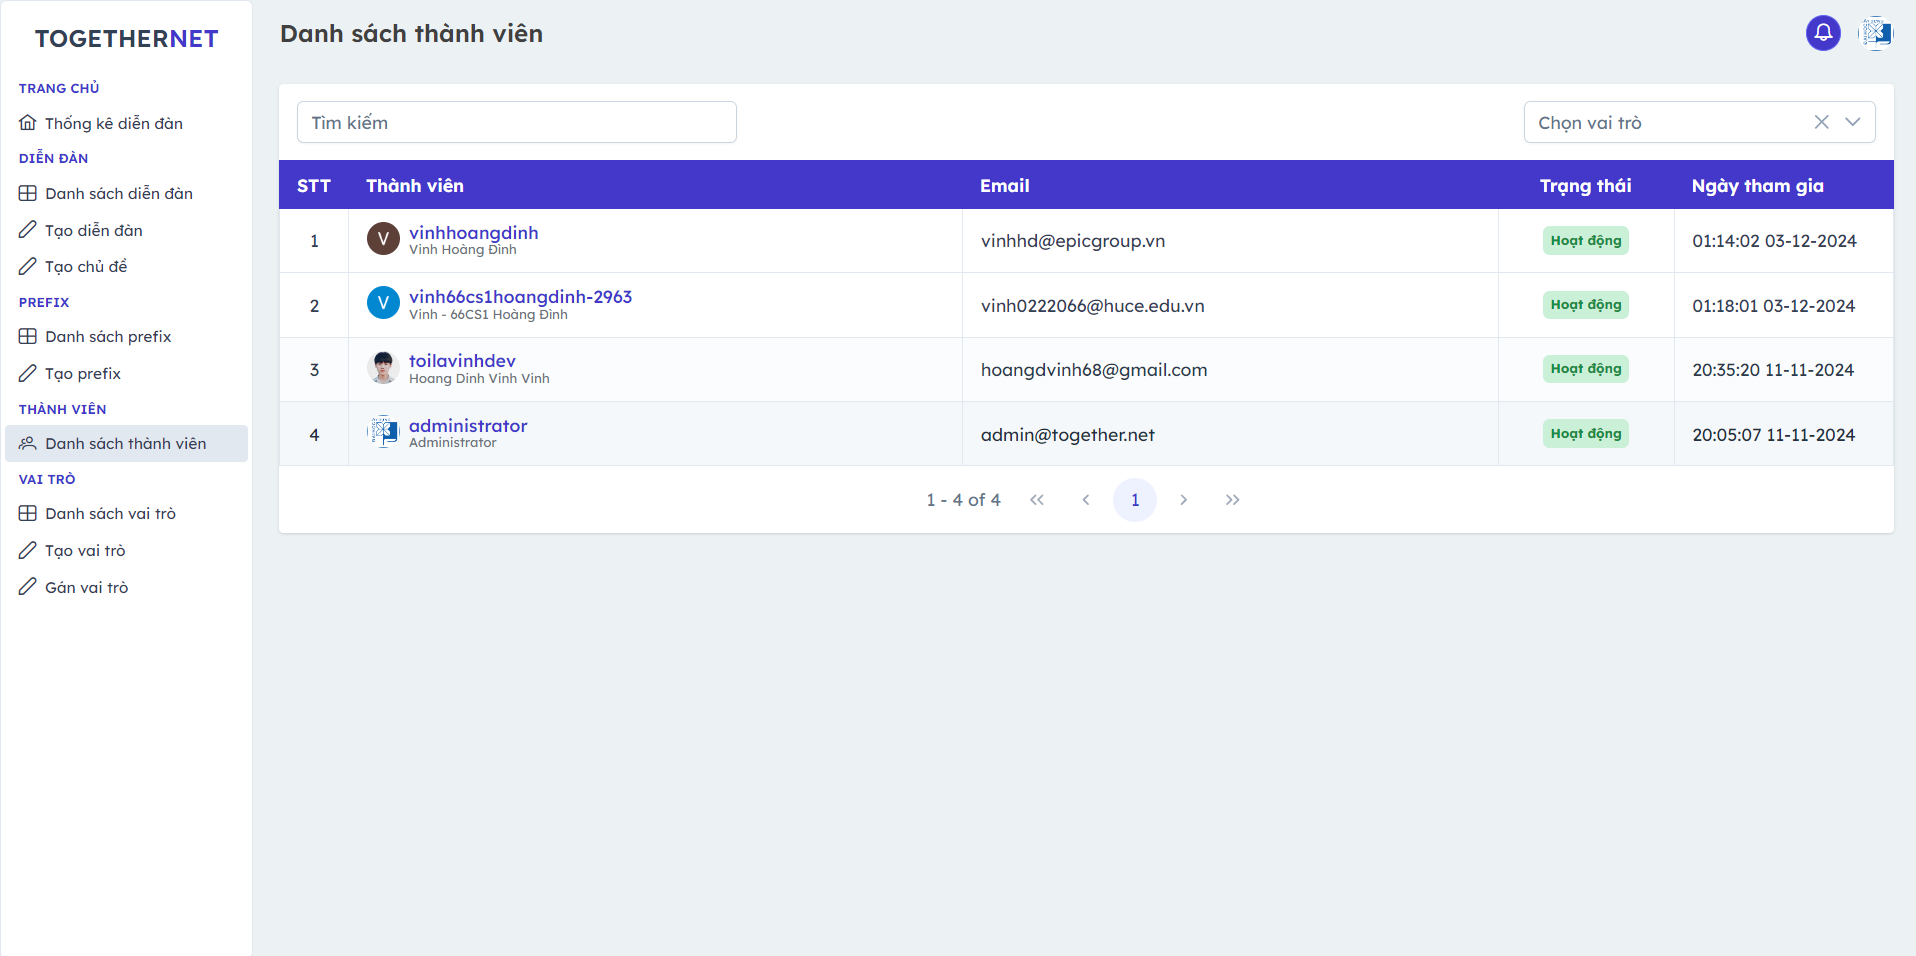
\includegraphics[width=1\linewidth]{figures/demo/management-user-page.png}
        \caption{UI Danh sách thành viên}
    \end{figure}
    
    \subsection{UI Danh sách vai trò}
    \begin{figure}[H]
        \centering
        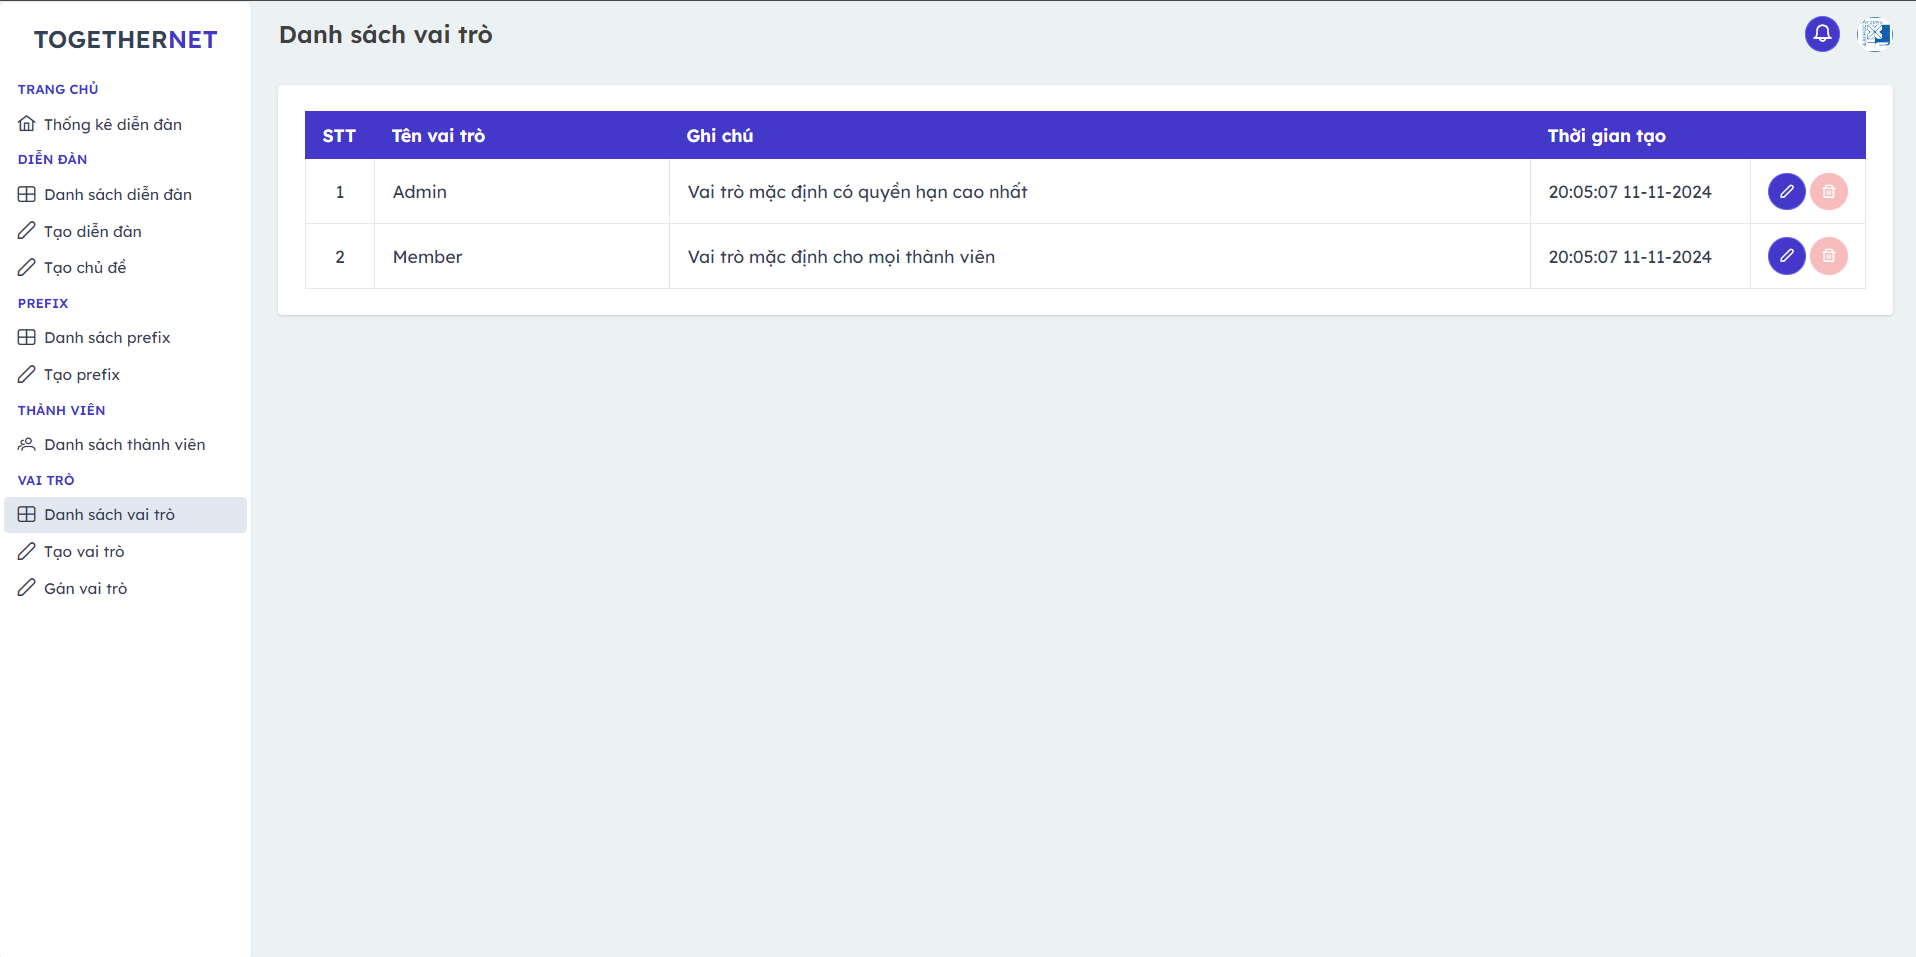
\includegraphics[width=1\linewidth]{figures/demo/management-role-page.png}
        \caption{UI Danh sách vai trò}
    \end{figure}

    \subsection{UI Cập nhật vai trò}
    \begin{figure}[H]
        \centering
        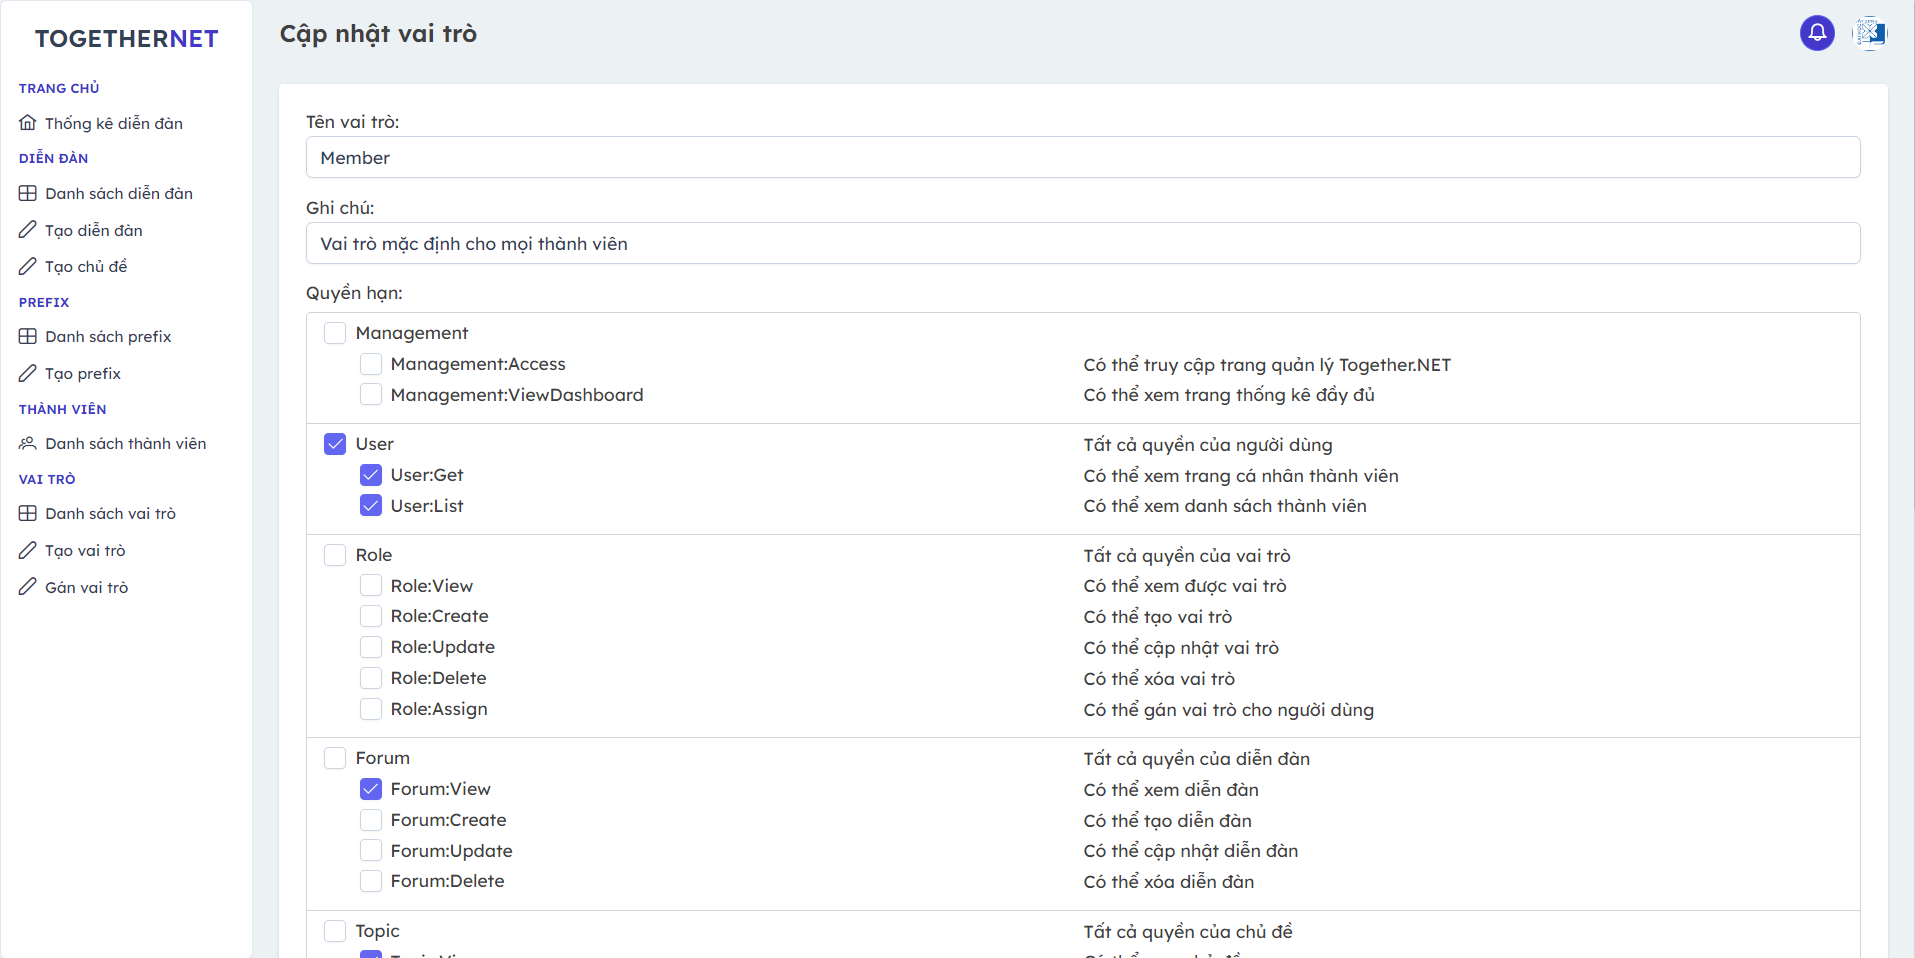
\includegraphics[width=1\linewidth]{figures/demo/management-role-update-page.png}
        \caption{UI Cập nhật vai trò}
    \end{figure}

    \subsection{UI Gán vai trò cho thành viên}
    \begin{figure}[H]
        \centering
        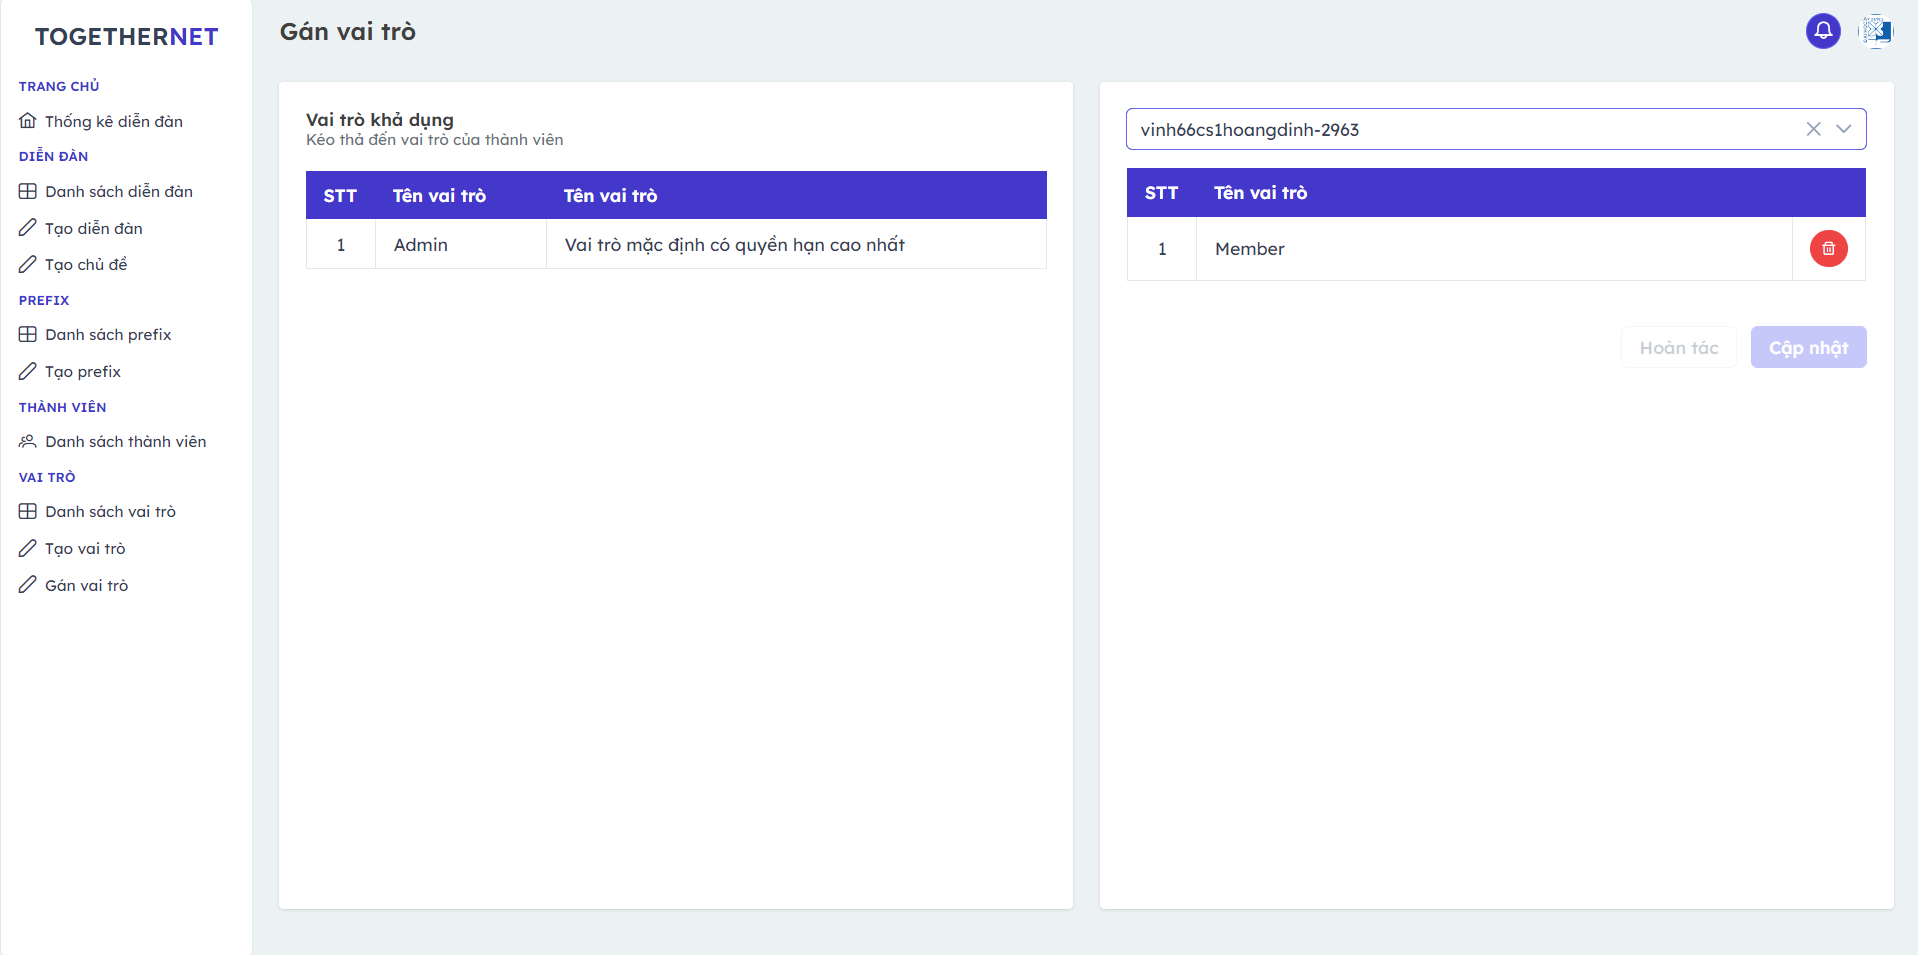
\includegraphics[width=1\linewidth]{figures/demo/management-role-assign.png}
        \caption{UI Gán vai trò cho thành viên}
    \end{figure}
    
\end{document}